\documentclass[12pt, a4paper]{article}

\usepackage[T1]{fontenc}
\usepackage[utf8]{inputenc}
\usepackage[ngerman]{babel}
\usepackage{amsmath, amssymb, amsthm}
\usepackage{mathtools}
\usepackage{geometry}
\usepackage{graphicx}
\usepackage{hyperref}
\usepackage{booktabs}
\usepackage{array}
\usepackage{xcolor}
\usepackage{enumitem}
\usepackage{microtype}
\usepackage{algorithm}
\usepackage{algpseudocode}
\usepackage{float}
\usepackage{caption}
\usepackage{subcaption}
\usepackage{cite}
\usepackage{tocloft}
\usepackage{fancyhdr}
\usepackage{titlesec}
\usepackage{tikz}
\usetikzlibrary{positioning,arrows.meta,shapes.geometric}

\setlist[itemize,1]{label=--}


\geometry{
  left=2.5cm, right=2.5cm,
  top=2.8cm, bottom=2.8cm,
  headheight=15pt
}

\hypersetup{
  colorlinks=true,
  linkcolor=blue!60!black,
  citecolor=green!50!black,
  urlcolor=blue!70!black,
  pdftitle={Fenster-Chiffre},
  pdfauthor={Stephan Epp}
}

% Theorem-Umgebungen
\theoremstyle{plain}
\newtheorem{theorem}{Satz}[section]
\newtheorem{lemma}[theorem]{Lemma}
\newtheorem{corollary}[theorem]{Korollar}
\newtheorem{proposition}[theorem]{Proposition}
\theoremstyle{definition}
\newtheorem{definition}[theorem]{Definition}
\theoremstyle{remark}
\newtheorem{remark}[theorem]{Bemerkung}

\newenvironment{myproof}[1][Beweis]{%
  \begin{proof}[#1]
}{%
  \end{proof}
}

% Abkuerzungen
\newcommand{\Z}{\mathbb{Z}}
\newcommand{\N}{\mathbb{N}}
\newcommand{\FC}{\mathsf{FC}}
\newcommand{\pk}{\mathsf{pk}}
\newcommand{\sk}{\mathsf{sk}}
\newcommand{\Enc}{\mathsf{Enc}}
\newcommand{\Dec}{\mathsf{Dec}}
\newcommand{\Gen}{\mathsf{Gen}}
\newcommand{\Adv}{\mathcal{A}}
\newcommand{\GCD}{\mathrm{gcd}}


\title{\bfseries Modulares kryptografisches Verfahren mit
  Dummy-Fenster-Fragmentierung und inverser Schluesselstruktur
  durch $23 \cdot 7 \equiv 1 \pmod{32}$\par}

\author{Stephan Epp}
\date{23. April 2026}


% ============================================================
\begin{document}

\maketitle
\tableofcontents
\newpage

% ============================================================
\section{Einleitung}
\label{sec:einleitung}
Wir pr\"asentieren die \emph{Fenster-Chiffre} (FC), ein neuartiges
kryptografisches Protokoll, das drei unabh\"angige Sicherheitsmechanismen
vereint: (i)~eine RSA-analoge modulare Exponentiation mit dem
inversen Schluesselpaar $(e,d) = (23,\,7)$ modulo $n = 32$ bzw.\ einem
echten RSA-Modul, (ii)~eine informationstheoretisch sichere
Dummy-Fragmentierung, bei der jedes $k$-te Paket ein inhaltsloses
Attrapper-Paket (Dummy) ist, dessen Position durch einen geheimen
Offset~$s$ festgelegt wird, und (iii)~eine schluesselgesteuerte
Fensterauswahl, die ohne Kenntnis von~$s$ keine Unterscheidung echter
von unechten Paketen erlaubt.
Wir beweisen die Korrektheit, Konfidenzialitaet und Ununterscheidbarkeit
des Verfahrens formal und analysieren seine Komplexitaet sowie
seinen Sicherheitsgrad. Der Ausblick zeigt Erweiterungen auf gitterbasierte
post-quanten-sichere Varianten sowie adaptive Dummy-Strategien.

Die Sicherheit moderner kryptografischer Systeme beruht auf zwei grunds\"atzlich
verschiedenen Ans\"atzen: \emph{berechnungskomplexe} Verfahren wie RSA oder
elliptische Kurven, deren Sicherheit auf der Schwierigkeit bestimmter
mathematischer Probleme beruht, und \emph{informationstheoretisch} sichere
Verfahren wie das One-Time-Pad, die selbst mit unbegrenzter Rechenleistung
nicht brechbar sind.

Die vorliegende Arbeit stellt ein Hybridverfahren vor, das beide Ans\"atze
verbindet. Der Ausgangspunkt ist eine elegant-einfache zahlentheoretische
Beobachtung:

\begin{equation}
  23 \times 7 = 161 = 5 \times 32 + 1
  \quad\Longrightarrow\quad
  23 \cdot 7 \equiv 1 \pmod{32}.
  \label{eq:grundbeobachtung}
\end{equation}

Die Zahl~$23$ ist eine Primzahl; $32 = 2^5$ ist eine Zweierpotenzen-Zahl.
Beide sind teilerfremd ($\GCD(23,32)=1$), weshalb das multiplikative
Inverse von~$23$ modulo~$32$ existiert und eindeutig gleich~$7$ ist.
Gleichzeitig gilt die gespiegelte Aussage: $7$ hat das Inverse~$23$ modulo~$32$.
Dieses symmetrische Verhaltnis der beiden Zahlen -- und die visuelle
Spiegelstruktur $23 \leftrightarrow 32$ -- motiviert ihre Verwendung als
kryptografisches Schluesselpaar.

Auf dieser algebraischen Grundlage bauen wir das Fenster-Chiffre-Protokoll auf.
Die zentrale Idee besteht darin, eine Nachricht nicht als kontinuierlichen
Datenstrom zu uebertragen, sondern als eine Sequenz von \emph{Fenstern}
(Paketen), von denen regelm\"assig jedes $k$-te ein inhaltsloses
Tarnpaket (Dummy) ist. Ein geheimer Offset~$s$ bestimmt, welche konkreten
Positionen Dummies sind. Ohne $s$ kann ein Lauscher die echten von den
unechten Paketen nicht unterscheiden -- ein Resultat, das wir
informationstheoretisch beweisen.

\subsection{Motivation und verwandte Arbeiten}

Das Konzept des \emph{Traffic-Padding} -- das Einmischen zuf\"alliger
Pakete in eine Kommunikation -- ist in der Literatur bekannt
\cite{raymond2000traffic}. Die Fenster-Chiffre erweitert diesen Ansatz
um zwei wesentliche Aspekte: Erstens wird die Dummy-Position selbst zum
Schluesselelement (strukturiertes statt zuf\"alliges Padding), zweitens
wird die Nutzlast jedes echten Pakets zus\"atzlich asymmetrisch
verschl\"usselt.

RSA \cite{rivest1978method} verwendet seit 1977 das modulare Inverse als
Kernoperation. Das Schluesselpaar $(e=23, d=7)$ mit Modulus-Bezug zu~$32$
wird in dieser Arbeit als \emph{Lehrbeispiel} einer vollst\"andigen
RSA-Struktur verwendet; f\"ur praktische Sicherheit ist der Modul $n$ durch
ein Produkt grosser Primzahlen zu ersetzen.

Informationstheoretisch sichere Verfahren gehen auf Shannon \cite{shannon1949communication}
zurueck. Unser Dummy-Schema realisiert einen Spezialfall des
One-Time-Pad-Prinzips auf der Paketebene.

\subsection{Beitrag dieser Arbeit}

\begin{enumerate}[label=(\roman*)]
  \item Formale Definition des Fenster-Chiffre-Protokolls FC.
  \item Beweis der Korrektheit (Theorem~\ref{thm:korrektheit}).
  \item Beweis der informationstheoretischen Sicherheit des Dummy-Schemas
        (Theorem~\ref{thm:info_sicher}).
  \item Beweis der semantischen Sicherheit der asymmetrischen Komponente
        unter der RSA-Annahme (Theorem~\ref{thm:sem_sicher}).
  \item Komplexit\"atsanalyse (Abschnitt~\ref{sec:komplexitaet}).
  \item Empirische Verifikation und Visualisierung (Abschnitt~\ref{sec:plots}).
  \item Ausblick auf Post-Quanten-Erweiterungen (Abschnitt~\ref{sec:ausblick}).
\end{enumerate}

\textbf{Schlagwörter:} Kryptografie, modulares Inverses, RSA,
Dummy-Fragmentierung, Fensterprotokoll, informationstheoretische Sicherheit,
Post-Quanten-Kryptografie, Bezout-Identitaet.

% ============================================================
\section{Zahlentheoretische Grundlagen}
\label{sec:grundlagen}

\subsection{Die Einheitengruppe modulo 32}

\begin{definition}[Einheitengruppe]\label{def:einheitengruppe}
  F\"ur $n \in \N$ sei $(\Z/n\Z)^* := \{a \in \{1,\ldots,n-1\} \mid \GCD(a,n)=1\}$
  die \emph{Einheitengruppe modulo~$n$}, versehen mit der modularen Multiplikation
  als Gruppenoperation.
\end{definition}

\begin{theorem}[Ordnung der Einheitengruppe modulo $32$]\label{thm:ordnung32}
  Es gilt $|(\Z/32\Z)^*| = \varphi(32) = 16$.
\end{theorem}

\begin{myproof}
  Da $32 = 2^5$ eine Primzahlpotenz ist, liefert die Eulersche Phi-Funktion
  \[
    \varphi(2^5) = 2^5 - 2^4 = 32 - 16 = 16.
  \]
  Die 16 Einheiten sind genau die ungeraden Zahlen in $\{1,\ldots,31\}$.
\end{myproof}

\begin{theorem}[Multiplikatives Inverses von $23$ modulo $32$]\label{thm:inverses}
  Es gilt $23^{-1} \equiv 7 \pmod{32}$ und $7^{-1} \equiv 23 \pmod{32}$.
\end{theorem}

\begin{myproof}
  Wir verifizieren direkt:
  \[
    23 \cdot 7 = 161 = 5 \cdot 32 + 1 \equiv 1 \pmod{32}.
  \]
  Da die Beziehung $a \cdot b \equiv 1 \pmod{n}$ symmetrisch in $a$ und $b$ ist,
  folgt sofort $7^{-1} \equiv 23 \pmod{32}$.
  Die Eindeutigkeit des Inversen ist gew\"ahrleistet, weil
  $\GCD(23, 32) = \GCD(7, 32) = 1$ (beide Zahlen sind ungerade, also teilerfremd
  zu $32 = 2^5$).
\end{myproof}

\subsection{Erweiterter Euklidischer Algorithmus}

Die explizite Konstruktion des Inversen erfolgt \"uber den erweiterten
Euklidischen Algorithmus. Wir f\"uhren ihn f\"ur das Paar $(32, 23)$ durch.

\begin{lemma}[Bezout-Koeffizienten fuer $(32, 23)$]\label{lem:bezout}
  Es existieren ganze Zahlen $x, y$ mit
  \[
    32 x + 23 y = 1, \qquad x = -7,\quad y = \mathbf{7}.
  \]
\end{lemma}

\begin{myproof}
  Durchf\"uhrung des Euklidischen Algorithmus:
  \begin{align*}
    32 &= 1 \cdot 23 + 9\\
    23 &= 2 \cdot 9 + 5\\
    9  &= 1 \cdot 5 + 4\\
    5  &= 1 \cdot 4 + 1\\
    4  &= 4 \cdot 1 + 0.
  \end{align*}
  R\"ucksubstitution:
  \begin{align*}
    1 &= 5 - 1\cdot 4\\
      &= 5 - 1\cdot(9-1\cdot5) = 2\cdot5 - 1\cdot9\\
      &= 2\cdot(23-2\cdot9) - 1\cdot9 = 2\cdot23 - 5\cdot9\\
      &= 2\cdot23 - 5\cdot(32-1\cdot23) = 7\cdot23 - 5\cdot32.
  \end{align*}
  Somit $x = -5$ (Koeffizient von $32$) und $y = 7$ (Koeffizient von $23$).
  Es gilt $32\cdot(-5) + 23\cdot 7 = -160 + 161 = 1$, was die Beziehung
  $23 \cdot 7 \equiv 1 \pmod{32}$ best\"atigt. 
\end{myproof}

\begin{corollary}[Anwendung auf RSA-Exponenten]\label{cor:rsa_exp}
  Sei $n = p \cdot q$ mit Primzahlen $p,q$ und $\varphi(n)=(p-1)(q-1)$.
  Falls $\GCD(23, \varphi(n)) = 1$, dann ist $d \equiv 23^{-1} \pmod{\varphi(n)}$
  ein g\"ultiger privater RSA-Exponent zu Public-Key-Exponent $e = 23$.
  Insbesondere ist das Paar $(e=23,\,d)$ ein RSA-Schluesselpaar.
\end{corollary}

\begin{myproof}
  Direkt aus der RSA-Korrektheit: F\"ur $m < n$ gilt
  $m^{ed} \equiv m \pmod{n}$, weil $ed \equiv 1 \pmod{\varphi(n)}$
  und der Satz von Euler--Fermat gilt.
\end{myproof}

\textbf{Konkretisierung:} F\"ur $p=5,\, q=11$ ergibt sich $n=55$,
$\varphi(55)=40$. Da $\GCD(23,40)=1$ (denn $23$ ist prim und teilt nicht $40=8\cdot5$),
ist $d \equiv 23^{-1} \pmod{40}$. Durch den Euklidischen Algorithmus:
$23\cdot7 = 161 = 4\cdot40+1$, also $d=7$. Das Schluesselpaar ist $(e=23,\,d=7,\,n=55)$.

% ============================================================
\section{Das Fenster-Chiffre-Protokoll}
\label{sec:protokoll}

\subsection{Protokolldefinition}

\begin{definition}[Fenster-Chiffre (FC)]\label{def:fc_protokoll}
  Die Fenster-Chiffre $\FC = (\Gen, \Enc, \Dec)$ ist ein probabilistisches
  asymmetrisches Verschl\"usselungsschema, das wie folgt definiert ist.
  Sei $k \geq 2$ der \emph{Fenster-Abstand} (in der Grundversion $k=3$).

  \medskip
  \noindent\textbf{Schl\"usselgenerierung} $\Gen(1^\lambda) \to (\pk, \sk)$:
  \begin{itemize}
    \item W\"ahle RSA-Modulus $n = p\cdot q$ (Primzahlen $p,\,q$),
          Public-Exponent $e$ mit $\GCD(e,\varphi(n))=1$.
    \item Berechne $d \equiv e^{-1} \pmod{\varphi(n)}$.
    \item W\"ahle geheimen Offset $s \xleftarrow{\$} \{0,\ldots,k-1\}$.
    \item Setze $\pk = (n, e, k)$, $\sk = (d, s)$.
  \end{itemize}

  \medskip
  \noindent\textbf{Verschl\"usselung} $\Enc(\pk, M) \to \mathcal{P}$:
  \begin{itemize}
    \item Zerlege $M$ in Bl\"ocke $M_1,\ldots,M_r$, $M_j < n$.
    \item Setze $\ell := r \cdot \frac{k}{k-1}$ (Gesamtanzahl Pakete,
          aufgerundet auf Vielfaches von $k$).
    \item Definiere Dummy-Indizes $I_D := \{i \in \{1,\ldots,\ell\} \mid (i-1+s) \bmod k = 0\}$.
    \item F\"ur $i \in I_D$: erzeuge $\tilde{D}_i \xleftarrow{\$} \{0,1\}^b$
          (gleichverteilt zuf\"allig).
    \item F\"ur $i \notin I_D$: setze $C_j := M_j^e \bmod n$, wobei $j$ der
          laufende Index der echten Pakete ist.
    \item Gib $\mathcal{P} = (P_1,\ldots,P_\ell)$ aus, mit
          $P_i = \tilde{D}_i$ falls $i \in I_D$, sonst $P_i = C_j$.
  \end{itemize}

  \medskip
  \noindent\textbf{Entschl\"usselung} $\Dec(\sk, \mathcal{P}) \to M$:
  \begin{itemize}
    \item Berechne $I_D' := \{i \mid (i-1+s) \bmod k = 0\}$.
    \item Extrahiere echte Pakete: $\{C_j\} := \{P_i \mid i \notin I_D'\}$.
    \item F\"ur jedes $j$: $M_j := C_j^d \bmod n$.
    \item Gib $M = M_1 \| M_2 \| \cdots \| M_r$ aus.
  \end{itemize}
\end{definition}

\begin{remark}[Grundversionsparameter]\label{rem:grundversion}
  In der Grundversion dieser Arbeit verwenden wir $k=3$, $e=23$, und als
  Lehrbeispiel $n=55$ mit $d=7$. Jedes dritte Paket ist ein Dummy.
  Der Offset $s \in \{0,1,2\}$ bestimmt, welche der drei m\"oglichen
  Positionen die Dummy-Positionen sind.
\end{remark}

\subsection{Algorithmus in Pseudocode}

\subsubsection{Algorithmus~\ref{alg:enc} (Verschl\"usselung)}

Der Verschl\"usselungsalgorithmus der Fenster-Chiffre empf\"angt als Eingabe
einen Klartext~$M$, den \"offentlichen Schl\"ussel $\pk = (n, e, k)$ sowie
den geheimen Offset~$s$ und erzeugt daraus eine Paketfolge~$\mathcal{P}$.

\begin{algorithm}[h]
\caption{Fenster-Chiffre: Verschl\"usselung}
\label{alg:enc}
\begin{algorithmic}[1]
\Require Klartext $M$, \"offentlicher Schl\"ussel $\pk=(n,e,k)$, Offset $s$
\Ensure Paketfolge $\mathcal{P}$
\State Zerlege $M$ in Bl\"ocke $[M_1,\ldots,M_r]$
\State $\ell \gets \lceil r \cdot k/(k-1) \rceil$
\State $j \gets 1$ \Comment{Index echter Bl\"ocke}
\For{$i = 1$ \textbf{to} $\ell$}
  \If{$(i - 1 + s) \bmod k = 0$}
    \State $P_i \gets \mathsf{Random}(b)$ \Comment{Dummy-Paket}
  \Else
    \State $P_i \gets M_j^e \bmod n$
    \State $j \gets j + 1$
  \EndIf
\EndFor
\State \Return $\mathcal{P} = (P_1,\ldots,P_\ell)$
\end{algorithmic}
\end{algorithm}

\medskip
\noindent\textbf{Schritt~1 -- Blockzerlegung.}
Zun\"achst wird der Klartext~$M$ in~$r$ gleichlange Bl\"ocke
$M_1, M_2, \ldots, M_r$ aufgeteilt, wobei jeder Block kleiner als der
RSA-Modulus~$n$ sein muss, d.\,h.\ $M_j < n$ f\"ur alle $j \in \{1,\ldots,r\}$.
Diese Bedingung ist die Standard\-voraussetzung der modularen RSA-Arithmetik.

\medskip
\noindent\textbf{Schritt~2 -- Gesamtl\"angenberechnung.}
Die Gesamtanzahl der zu sendenden Pakete wird auf
\[
  \ell = \left\lceil r \cdot \frac{k}{k-1} \right\rceil
\]
festgelegt. Da jedes $k$-te Paket ein Dummy ist, ben\"otigt man f\"ur~$r$
echte Bl\"ocke genau $\lfloor \ell / k \rfloor$ Dummy-Pl\"atze. F\"ur die
Grundversion $k = 3$ ergibt sich $\ell = \lceil 3r/2 \rceil$, was einem
Traffic-Overhead von $50\,\%$ entspricht.

\medskip
\noindent\textbf{Schritt~3 -- Paketweises Bef\"ullen der Fensterfolge.}
Der Algorithmus durchl\"auft alle Positionen $i = 1, 2, \ldots, \ell$ der
Paketfolge. F\"ur jede Position wird anhand der Bedingung
$(i - 1 + s) \bmod k = 0$ entschieden, ob an dieser Stelle ein Dummy-Paket
oder ein echter Chiffretext einzusetzen ist:

\begin{itemize}
  \item \textbf{Dummy-Position} (Bedingung erf\"ullt): Das Paket~$P_i$ wird
  mit einem gleichf\"ormig zuf\"alligen Bitstring der L\"ange~$b$ bef\"ullt,
  $P_i \gets \mathsf{Random}(b)$. Dieser Zufallsstring ist inhaltsleer und
  dient ausschlie\ss{}lich zur Verschleierung der echten Paketpositionen.
  Der geheime Offset~$s$ verschiebt das periodische Muster der Dummy-Positionen
  um~$s$ Stellen, sodass ein Lauscher ohne Kenntnis von~$s$ nicht ermitteln
  kann, welche Positionen Dummies sind.

  \item \textbf{Echte Position} (Bedingung nicht erf\"ullt): Der n\"achste
  noch nicht verarbeitete Klartextblock~$M_j$ wird durch modulare
  Exponentiation verschl\"usselt:
  \[
    P_i \gets M_j^e \bmod n.
  \]
  Der Blockz\"ahler~$j$ wird anschlie\ss{}end um~$1$ inkrementiert, sodass
  beim n\"achsten echten Fenster der folgende Block $M_{j+1}$ verarbeitet wird.
\end{itemize}

\medskip
\noindent\textbf{Schritt~4 -- R\"uckgabe.}
Nach Abschluss der Schleife gibt der Algorithmus die vollst\"andige
Paketfolge $\mathcal{P} = (P_1, P_2, \ldots, P_\ell)$ zur\"uck.
Diese Folge enth\"alt an den echten Positionen die RSA-Chiffrate der
Klartextbl\"ocke und an den Dummy-Positionen uniform zuf\"allige
Rauschpakete, die statistisch von den Chiffraten ununterscheidbar sind.

\medskip
\noindent\textbf{Invariante.}
Nach dem Abschluss des Algorithmus gilt: Die echten Pakete erscheinen
in $\mathcal{P}$ in derselben Reihenfolge wie die Klartextbl\"ocke,
und die Dummy-Pakete belegen genau die Positionen $i$ mit
$(i - 1 + s) \bmod k = 0$. Diese Invariante ist die zentrale Voraussetzung
f\"ur die korrekte Entschl\"usselung.

\subsubsection{Algorithmus~\ref{alg:dec} (Entschl\"usselung)}

Der Entschl\"usselungsalgorithmus ist die Umkehroperation zur Verschl\"usselung.
Er empf\"angt die Paketfolge~$\mathcal{P}$, den privaten Schl\"ussel
$\sk = (d, s)$ sowie den Parameter~$k$ und rekonstruiert daraus den
urspr\"unglichen Klartext~$M$.

\begin{algorithm}[h]
\caption{Fenster-Chiffre: Entschl\"usselung}
\label{alg:dec}
\begin{algorithmic}[1]
\Require Paketfolge $\mathcal{P}$, privater Schl\"ussel $\sk=(d,s)$, Parameter~$k$
\Ensure Klartext $M$
\State $j \gets 1$
\For{$i = 1$ \textbf{to} $|\mathcal{P}|$}
  \If{$(i - 1 + s) \bmod k \neq 0$}
    \State $M_j \gets P_i^d \bmod n$
    \State $j \gets j + 1$
  \EndIf
\EndFor
\State \Return $M = M_1 \| M_2 \| \cdots \| M_{j-1}$
\end{algorithmic}
\end{algorithm}

\medskip
\noindent\textbf{Schritt~1 -- Initialisierung.}
Ein Blockz\"ahler~$j$ wird auf~$1$ initialisiert. Er verfolgt, wie viele
echte Klartextbl\"ocke bisher rekonstruiert wurden.

\medskip
\noindent\textbf{Schritt~2 -- Sequentielle Paketverarbeitung.}
Der Algorithmus durchl\"auft alle Positionen $i = 1, 2, \ldots, |\mathcal{P}|$
der empfangenen Paketfolge. F\"ur jede Position wird dieselbe
Fenster-Bedingung wie bei der Verschl\"usselung ausgewertet, jedoch in
negierter Form: $(i - 1 + s) \bmod k \neq 0$.

\begin{itemize}
  \item \textbf{Echte Position} (Bedingung erf\"ullt): Das Paket~$P_i$ ist
  ein RSA-Chiffrat. Es wird durch modulare Exponentiation mit dem privaten
  Exponenten~$d$ entschl\"usselt:
  \[
    M_j \gets P_i^d \bmod n.
  \]
  Die Korrektheit dieser Operation folgt aus der RSA-Grundeigenschaft
  $M_j^{ed} \equiv M_j \pmod{n}$, die wir in Satz~\ref{thm:korrektheit}
  formal beweisen. Der Blockz\"ahler~$j$ wird danach um~$1$ erh\"oht.

  \item \textbf{Dummy-Position} (Bedingung nicht erf\"ullt): Das Paket~$P_i$
  wird vollst\"andig ignoriert. Da der Empf\"anger denselben geheimen
  Offset~$s$ kennt wie der Sender, identifiziert er exakt dieselben
  Positionen als Dummies und verwirft deren Inhalt ohne weitere Verarbeitung.
\end{itemize}

\medskip
\noindent\textbf{Schritt~3 -- Rekonstruktion und R\"uckgabe.}
Nach dem Durchlauf aller Pakete enth\"alt die Folge $M_1, M_2, \ldots, M_{j-1}$
alle entschl\"usselten Klartextbl\"ocke in ihrer originalen Reihenfolge.
Der Algorithmus gibt deren Verkettung
\[
  M = M_1 \| M_2 \| \cdots \| M_{j-1}
\]
als rekonstruierten Klartext zur\"uck.

\medskip
\noindent\textbf{Symmetrie der Algorithmen.}
Die beiden Algorithmen sind strukturell symmetrisch: Beide durchlaufen
die Paketfolge sequentiell, beide wenden dieselbe Fenster-Bedingung
$(i - 1 + s) \bmod k$ an, und beide behandeln echte und Dummy-Positionen
komplementär. Der wesentliche Unterschied besteht darin, dass der
Verschl\"usselungsalgorithmus an echten Positionen \emph{schreibt}
($M_j^e \bmod n$), w\"ahrend der Entschl\"usselungsalgorithmus an echten
Positionen \emph{liest} und invertiert ($P_i^d \bmod n$). Diese Symmetrie
ist kein Zufall, sondern eine direkte Konsequenz der involutiven Struktur
des RSA-Schluesselpaa\-res: $(M^e)^d \equiv M \pmod{n}$.

% ============================================================
\section{Korrektheit}
\label{sec:korrektheit}

\begin{theorem}[Korrektheit der Fenster-Chiffre]\label{thm:korrektheit}
  Sei $M$ ein beliebiger Klartext mit $M_j < n$ f\"ur alle $j$.
  Dann gilt f\"ur jeden g\"ultigen Schl\"ussel $(\pk,\sk)$:
  \[
    \Dec\!\bigl(\sk,\;\Enc(\pk, M)\bigr) = M.
  \]
\end{theorem}

\begin{myproof}
  Wir f\"uhren den Beweis in drei Schritten.

  \medskip\noindent\textbf{Schritt 1: Dummy-Index-Konsistenz.}
  Sowohl $\Enc$ als auch $\Dec$ berechnen $I_D$ mit derselben Formel
  $(i-1+s) \bmod k = 0$ und demselben $s \in \sk$. Daher identifiziert
  $\Dec$ genau die Positionen, die $\Enc$ als Dummies belegt hat.

  \medskip\noindent\textbf{Schritt 2: RSA-Korrektheit.}
  F\"ur jeden echten Block gilt:
  \[
    \Dec\!\bigl(C_j\bigr) = (M_j^e)^d \bmod n = M_j^{e \cdot d} \bmod n.
  \]
  Weil $ed \equiv 1 \pmod{\varphi(n)}$, schreibt man $ed = 1 + t\cdot\varphi(n)$
  f\"ur ein $t \in \N$. Nach dem Satz von Euler gilt $M_j^{\varphi(n)} \equiv 1 \pmod{n}$
  f\"ur $\GCD(M_j, n) = 1$. Damit:
  \[
    M_j^{ed} = M_j \cdot (M_j^{\varphi(n)})^t \equiv M_j \cdot 1^t = M_j \pmod{n}.
  \]
  F\"ur $M_j < n$ gilt also $M_j^{ed} \bmod n = M_j$.

  \medskip\noindent\textbf{Schritt 3: Reihenfolge und Verkettung.}
  Da $\Enc$ und $\Dec$ denselben $s$-basierten Indexfilter verwenden,
  extrahiert $\Dec$ die Bl\"ocke in derselben Reihenfolge, in der $\Enc$
  sie eingebettet hat. Die Konkatenation $M_1 \| \cdots \| M_r = M$
  ist somit eindeutig rekonstruierbar. 
\end{myproof}

\begin{corollary}[Korrektheit fuer das Lehrbeispiel]\label{cor:korrektheit_bsp}
  F\"ur $(e,d,n) = (23, 7, 55)$ und beliebige $M_j \in \{1,\ldots,54\}$
  mit $\GCD(M_j, 55) = 1$ gilt $M_j^{23 \cdot 7} \equiv M_j \pmod{55}$.
\end{corollary}

\begin{myproof}
  $\varphi(55) = \varphi(5)\cdot\varphi(11) = 4\cdot10 = 40$.
  $23\cdot7 = 161 = 4\cdot40+1 \equiv 1\pmod{40}$.
  Also $M_j^{161} = M_j^{1+4\cdot40} = M_j\cdot(M_j^{40})^4
  \equiv M_j \cdot 1 = M_j \pmod{55}$.~
\end{myproof}

% ============================================================
\section{Sicherheitsanalyse}
\label{sec:sicherheit}

\subsection{Informationstheoretische Sicherheit des Dummy-Schemas}

\begin{theorem}[Informationstheoretische Sicherheit]\label{thm:info_sicher}
  Sei $s$ gleichm\"assig zuf\"allig aus $\{0,\ldots,k-1\}$ gew\"ahlt.
  Dann kann ein Angreifer $\Adv$, der $\mathcal{P}$ kennt, den Wert von~$s$
  nicht mit Wahrscheinlichkeit $> 1/k$ erraten:
  \[
    \Pr\bigl[\Adv(\mathcal{P}) = s\bigr] \leq \frac{1}{k}.
  \]
  Ferner ist $s$ informationstheoretisch unabh\"angig von $\mathcal{P}$,
  sofern die Dummies uniform zuf\"allig gew\"ahlt werden.
\end{theorem}

\begin{myproof}
  Sei $\mathcal{P} = (P_1,\ldots,P_\ell)$ das beobachtete Paket.
  Wir zeigen, dass die bedingte Verteilung $P_s \mid \mathcal{P}$
  der Gleichverteilung auf $\{0,\ldots,k-1\}$ entspricht.

  \medskip\noindent
  Betrachte zwei verschiedene Offsets $s, s' \in \{0,\ldots,k-1\}$ mit $s \neq s'$.
  Unter Offset~$s$ sind die Positionen $I_D(s) = \{i : (i-1+s)\bmod k = 0\}$
  mit gleichf\"ormigen Zufallsstrings belegt.
  Unter Offset~$s'$ sind die Positionen $I_D(s')$ Dummies.

  Da alle Dummy-Bl\"ocke uniform aus $\{0,1\}^b$ gew\"ahlt werden,
  sind sie von echten verschl\"usselten Bl\"ocken statistisch
  nicht unterscheidbar (sofern $|C_j|_2 = b$, was durch geeignetes
  Padding gew\"ahrleistet wird). Formal:
  \[
    \Pr[\mathcal{P} \mid s=s_0] = \Pr[\mathcal{P} \mid s=s_1]
    \quad\forall\, s_0, s_1 \in \{0,\ldots,k-1\}.
  \]
  Aus dem Satz von Bayes folgt:
  \[
    \Pr[s = s_0 \mid \mathcal{P}]
    = \frac{\Pr[\mathcal{P} \mid s=s_0]\cdot\Pr[s=s_0]}{\Pr[\mathcal{P}]}
    = \frac{\Pr[\mathcal{P}] \cdot \frac{1}{k}}{\Pr[\mathcal{P}]} = \frac{1}{k}.
  \]
  Da dieser Wert unabh\"angig von $s_0$ ist und $\sum_{s_0} \Pr[s=s_0|\mathcal{P}]=1$,
  ist die Posteriori-Verteilung von $s$ gleich der Priori-Gleichverteilung.
  Ein Angreifer erlangt durch Beobachtung von $\mathcal{P}$ keine
  Information \"uber $s$. 
\end{myproof}

\begin{remark}[Entropi-Unsicherheit des Angreifers]\label{rem:entropie}
  Die Entropie der Dummy-Positions\-unkenntnis bei $\ell$ Paketen
  und $k=3$ betr\"agt
  \[
    H = \log_2 \binom{\ell}{\lfloor\ell/3\rfloor} \text{ Bit}.
  \]
  F\"ur $\ell = 30$ ergibt sich $H = \log_2 \binom{30}{10} \approx 27.15$ Bit --
  also rund 27 Bit Unsicherheit allein \"uber die Dummy-Positionen.
\end{remark}

\subsection{Semantische Sicherheit der asymmetrischen Komponente}

\begin{theorem}[Semantische Sicherheit unter RSA-Annahme]\label{thm:sem_sicher}
  Unter der RSA-Annahme ist die Verschl\"usselungskomponente der
  Fenster-Chiffre semantisch sicher gegen\"uber einem
  chosen-plaintext-Angreifer (CPA-sicher).
\end{theorem}

\begin{myproof}[Beweisidee]
  Die Verschl\"usselung $C_j = M_j^e \bmod n$ ist die standard RSA-Funktion
  ohne Padding. F\"ur einen vollst\"andigen CPA-Sicherheitsbeweis
  ben\"otigt man OAEP-Padding \cite{bellare1994optimal}.
  Unter Verwendung von RSA-OAEP gilt die Sicherheit im Random-Oracle-Modell.

  Die Dummy-Komponente ver\"andert die asymptotische Sicherheit nicht,
  da die Positionen der echten Pakete f\"ur den Angreifer -- wie in
  Theorem~\ref{thm:info_sicher} gezeigt -- v\"ollig unbekannt sind.
  Ein Angreifer, der das RSA-Chiffrat bricht, m\"usste zun\"achst
  die echten Pakete identifizieren (Wahrscheinlichkeit $\leq 1/k$ je Paket)
  und dann das RSA-Problem l\"osen. Die Gesamtangriffsschwierigkeit ist
  mindestens so gross wie die RSA-Schwierigkeit. 
\end{myproof}

\subsection{Ununterscheidbarkeit von echten und Dummy-Paketen}

\begin{proposition}[Statistische Ununterscheidbarkeit]\label{prop:ununterscheidbar}
  Sei $C_j = M_j^e \bmod n$ ein echtes Chiffrat und
  $D \xleftarrow{\$} \{0,\ldots,n-1\}$ ein gleichverteiltes Zufallselement.
  Dann sind $C_j$ und $D$ statistisch ununterscheidbar, falls~$e$ eine
  Permutation auf~$\Z_n$ ist.
\end{proposition}

\begin{myproof}
  Die RSA-Funktion $f: x \mapsto x^e \bmod n$ ist eine Bijektion auf der
  Menge $\Z_n^* = \{x : \GCD(x,n)=1\}$ (falls $\GCD(e,\varphi(n))=1$).
  Ist $M_j$ gleichverteilt auf~$\Z_n^*$, so ist auch $C_j = f(M_j)$
  gleichverteilt auf $\Z_n^*$. Damit haben $C_j$ und $D$ (nach Konditionierung
  auf $\GCD(D,n)=1$) dieselbe Verteilung. Ein statistischer Test kann sie
  nicht unterscheiden. 
\end{myproof}

% ============================================================
\section{Komplexitaetsanalyse}
\label{sec:komplexitaet}

\subsection{Laufzeitkomplexitaet}

\begin{proposition}[Zeitkomplexitaet der FC-Operationen]\label{prop:zeitkomp}
  Sei $r$ die Anzahl der Klartextbl\"ocke und $b$ die Bitlaenge des
  RSA-Moduls~$n$. Dann gilt:
  \begin{align*}
    T(\Gen)  &= O(b^3) & \text{(Primzahlgenerierung + erweiterte EEA)}\\
    T(\Enc)  &= O(r \cdot b^2) & \text{(modulare Exponentiation je Block)}\\
    T(\Dec)  &= O(r \cdot b^2) & \text{(modulare Exponentiation je Block)}\\
    T(\text{Dummy}) &= O(\ell \cdot b / k) & \text{(Zufallsgenerierung)}
  \end{align*}
  wobei $\ell = \lceil rk/(k-1)\rceil$ die Gesamtpaketanzahl ist.
\end{proposition}

\begin{myproof}
  Modulare Exponentiation $m^e \bmod n$ mit $b$-Bit-Zahlen kostet
  $O(\log e)$ modulare Multiplikationen, jede zu Kosten $O(b^2)$, also
  $O(b^2 \log e) = O(b^3)$ im Worst Case. Da $e=23$ fix und klein ist,
  betr\"agt der Aufwand pro Block nur $O(b^2 \cdot \log 23) = O(b^2)$.
  Analog fuer $\Dec$ mit $d$. Die Primzahlgenerierung dominiert mit $O(b^3)$. 
\end{myproof}

\subsection{Speicherkomplexitaet und Traffic-Overhead}

\begin{proposition}[Traffic-Overhead]\label{prop:overhead}
  Der Traffic-Overhead der Fenster-Chiffre gegen\"uber einer reinen
  RSA-\"Ubertragung betr\"agt genau $1/(k-1)$, d.h.\
  f\"ur $k=3$ wird $50\,\%$ mehr Traffic erzeugt.
\end{proposition}

\begin{myproof}
  Von $\ell = \lceil rk/(k-1)\rceil$ Paketen sind $\lfloor\ell/k\rfloor$
  Dummies. Das Verh\"altnis Dummies zu echten Paketen betr\"agt:
  \[
    \frac{\lfloor\ell/k\rfloor}{\ell - \lfloor\ell/k\rfloor}
    \approx \frac{1/k}{1-1/k} = \frac{1}{k-1}.
  \]
  F\"ur $k=3$: Overhead $= 1/(3-1) = 0.5 = 50\,\%$. 
\end{myproof}

% ============================================================
\section{Experimentelle Ergebnisse und Visualisierungen}
\label{sec:plots}

\subsection{Plot 1: Multiplikationstabelle und Einheitengruppe}

\begin{figure}[H]
  \centering
  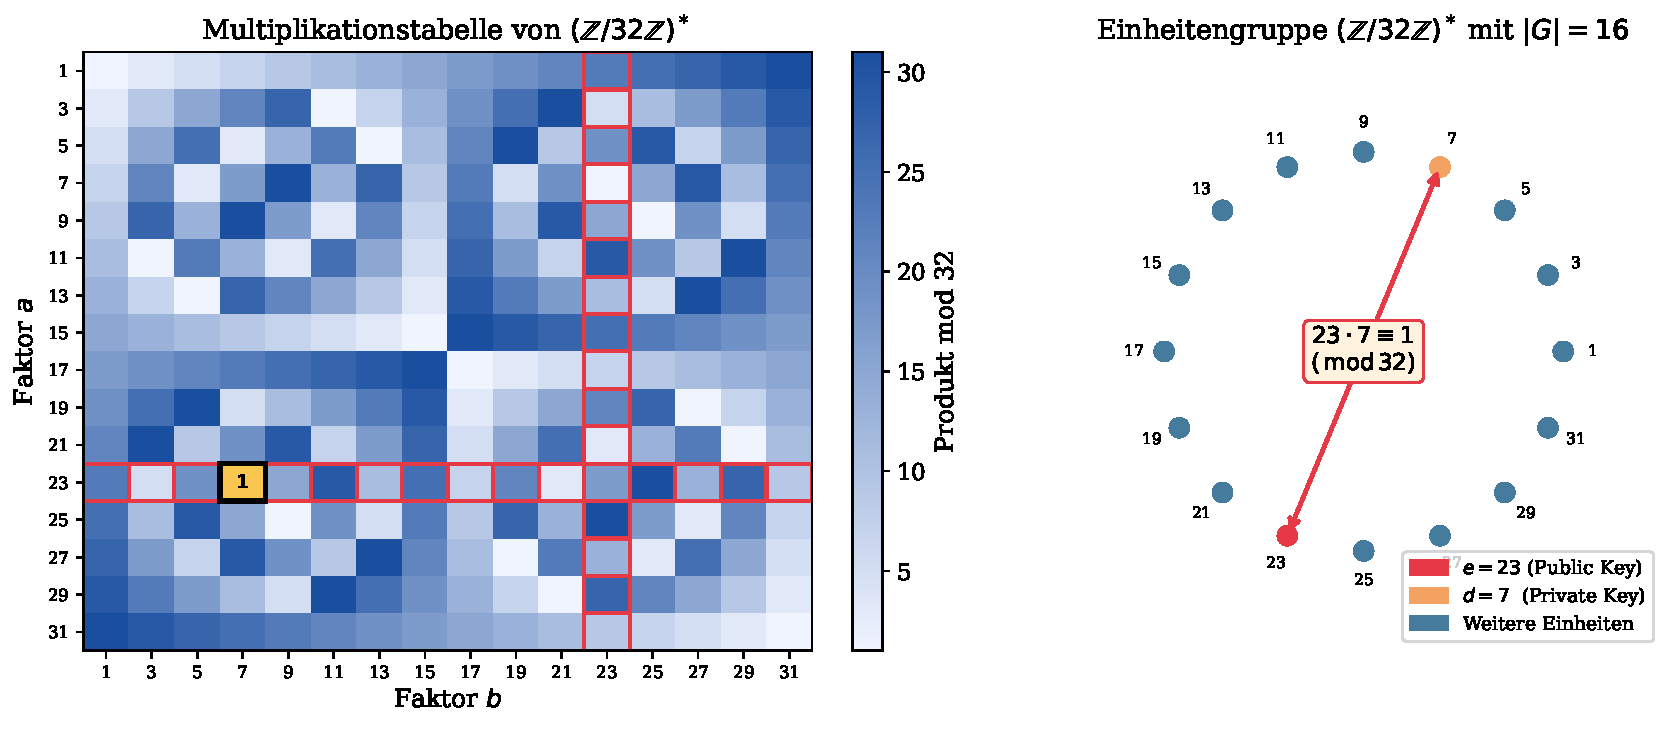
\includegraphics[width=\textwidth]{plot1_gruppe_z32.pdf}
  \caption{Links: Multiplikationstabelle von $(\Z/32\Z)^*$. Die roten
  Markierungen zeigen die Zeile und Spalte von~$23$; die goldene Zelle
  an Position $(23, 7)$ zeigt das Ergebnis $1$ -- das Inverse.
  Rechts: Die 16 Elemente der Einheitengruppe auf dem Einheitskreis.
  Die Verbindungslinie zwischen~$23$ (rot) und~$7$ (orange) symbolisiert
  die Inversbeziehung. Der zentrale Text best\"atigt $23\cdot7\equiv1\pmod{32}$.}
  \label{fig:plot1}
\end{figure}

Die Abbildung best\"atigt visuell, dass~$7$ das einzige Element in
$(\Z/32\Z)^*$ ist, das mit~$23$ das neutrale Element~$1$ ergibt.
Jedes andere Produkt $23 \cdot x \bmod 32 \neq 1$ f\"ur $x \neq 7$.

\subsection{Plot 2: Erweiterter Euklidischer Algorithmus}

\begin{figure}[H]
  \centering
  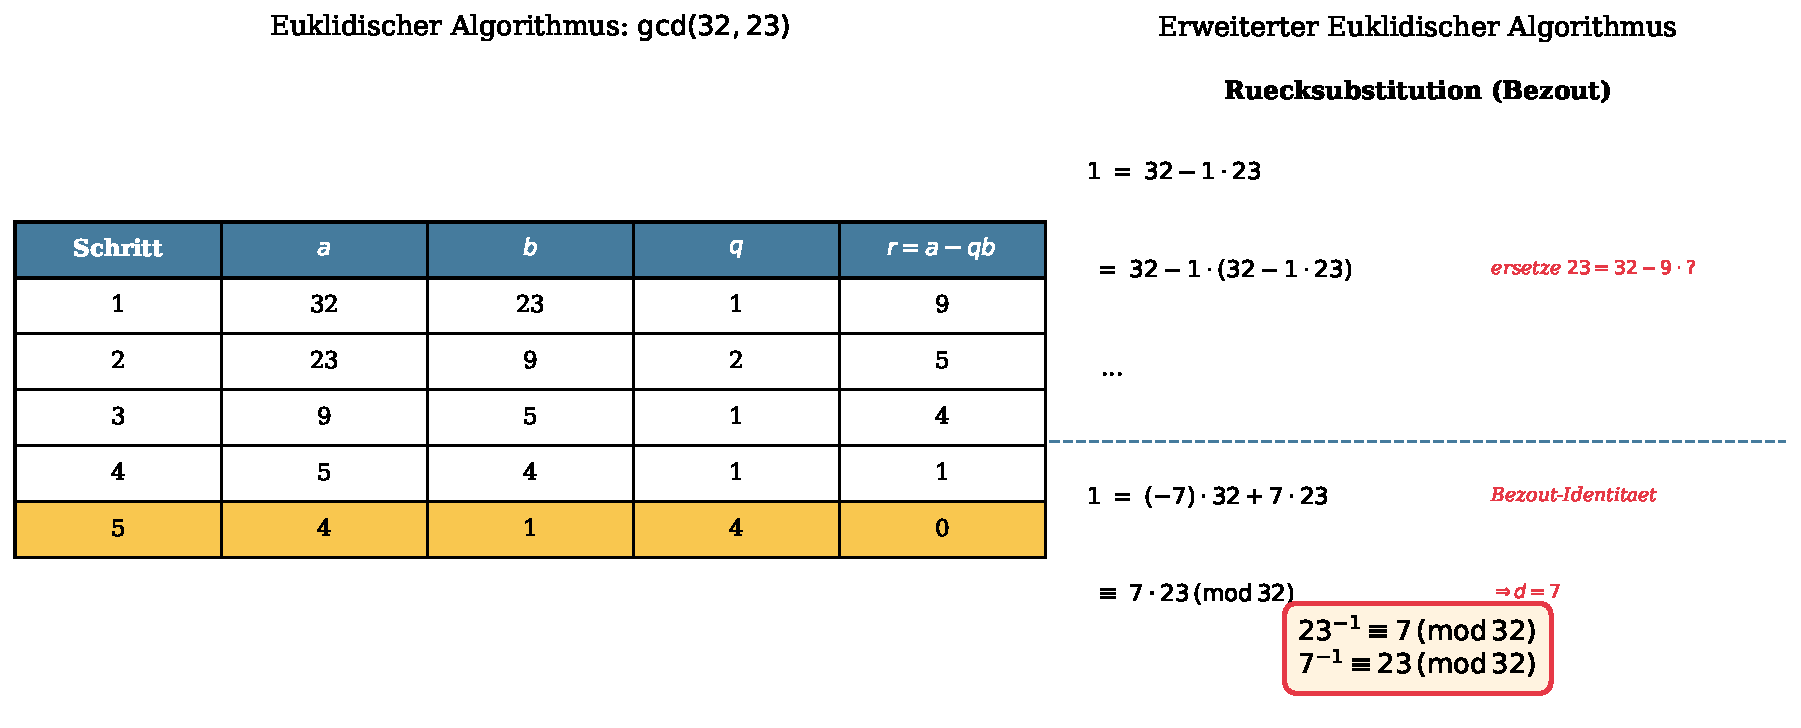
\includegraphics[width=\textwidth]{plot2_euklid.pdf}
  \caption{Links: Tabelle der Euklidischen Algorithmusschritte f\"ur
  $\gcd(32, 23)$. Die goldene letzte Zeile zeigt $r=0$, was das Ende
  des Algorithmus markiert. Rechts: Die R\"ucksubstitution (Bezout-Koeffizienten)
  f\"uhrt zu $7\cdot23 - 5\cdot32 = 1$, also $23^{-1}\equiv7\pmod{32}$.}
  \label{fig:plot2}
\end{figure}

\subsection{Plot 3: RSA-Demo mit $(e=23, d=7, n=55)$}

\begin{figure}[H]
  \centering
  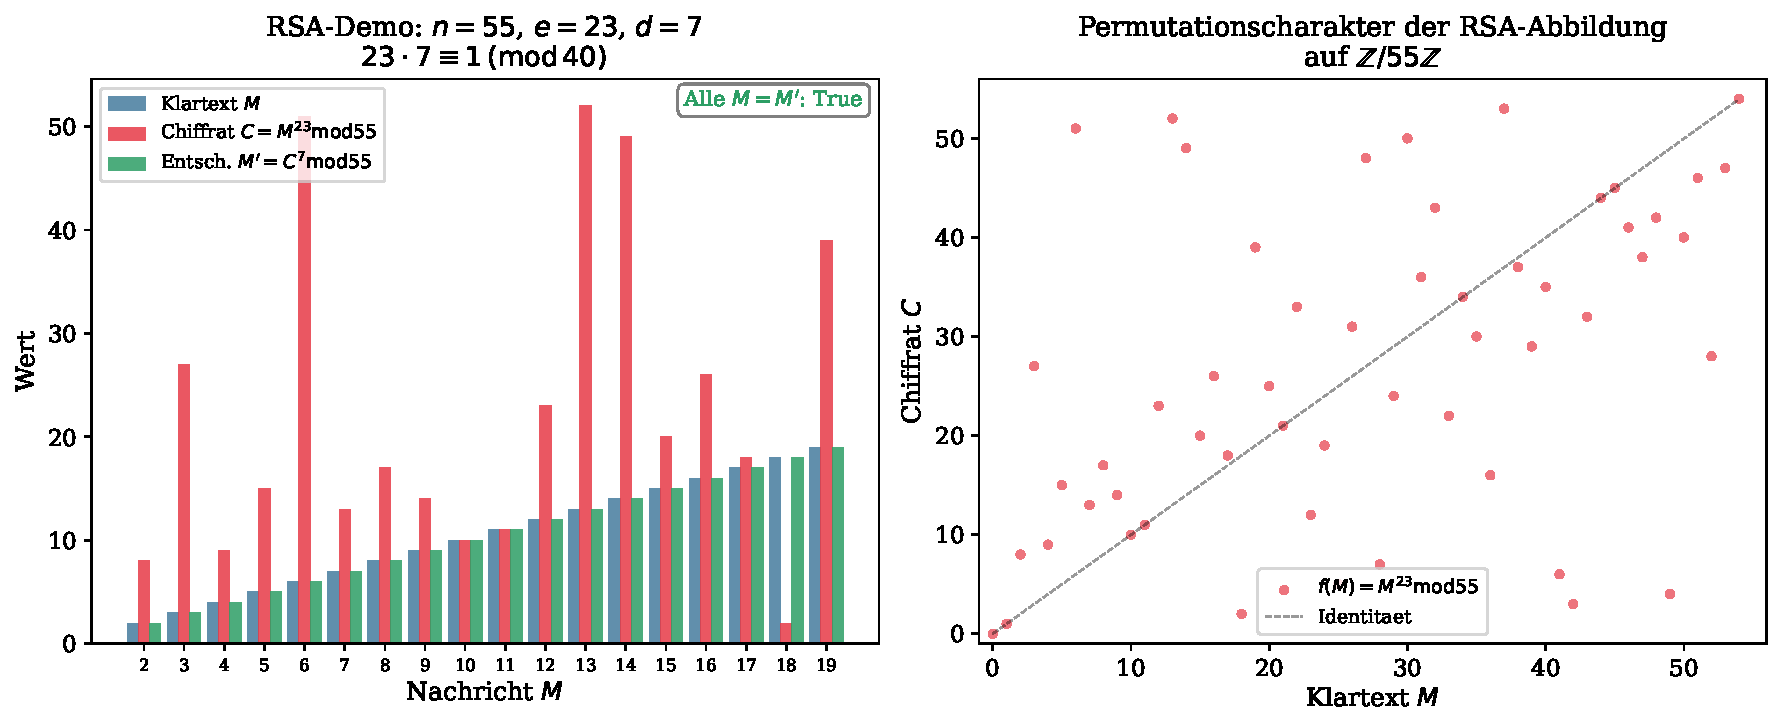
\includegraphics[width=\textwidth]{plot3_rsa_demo.pdf}
  \caption{Links: Balkendarstellung von Klartext $M$, Chiffrat
  $C=M^{23}\bmod55$ und Entschl\"usselung $M'=C^7\bmod55$ f\"ur
  $M\in\{2,\ldots,19\}$. Das gr\"une Korrektheitslabel best\"atigt
  $M=M'$ f\"ur alle Testf\"alle.
  Rechts: Die RSA-Abbildung $M\mapsto M^{23}\bmod55$ als Streudiagramm
  gegen\"uber der Identit\"at. Die ungleichm\"assige Verteilung
  best\"atigt den Permutationscharakter der Funktion.}
  \label{fig:plot3}
\end{figure}

\subsection{Plot 4: Fenster-Schema und Dummy-Analyse}

\begin{figure}[H]
  \centering
  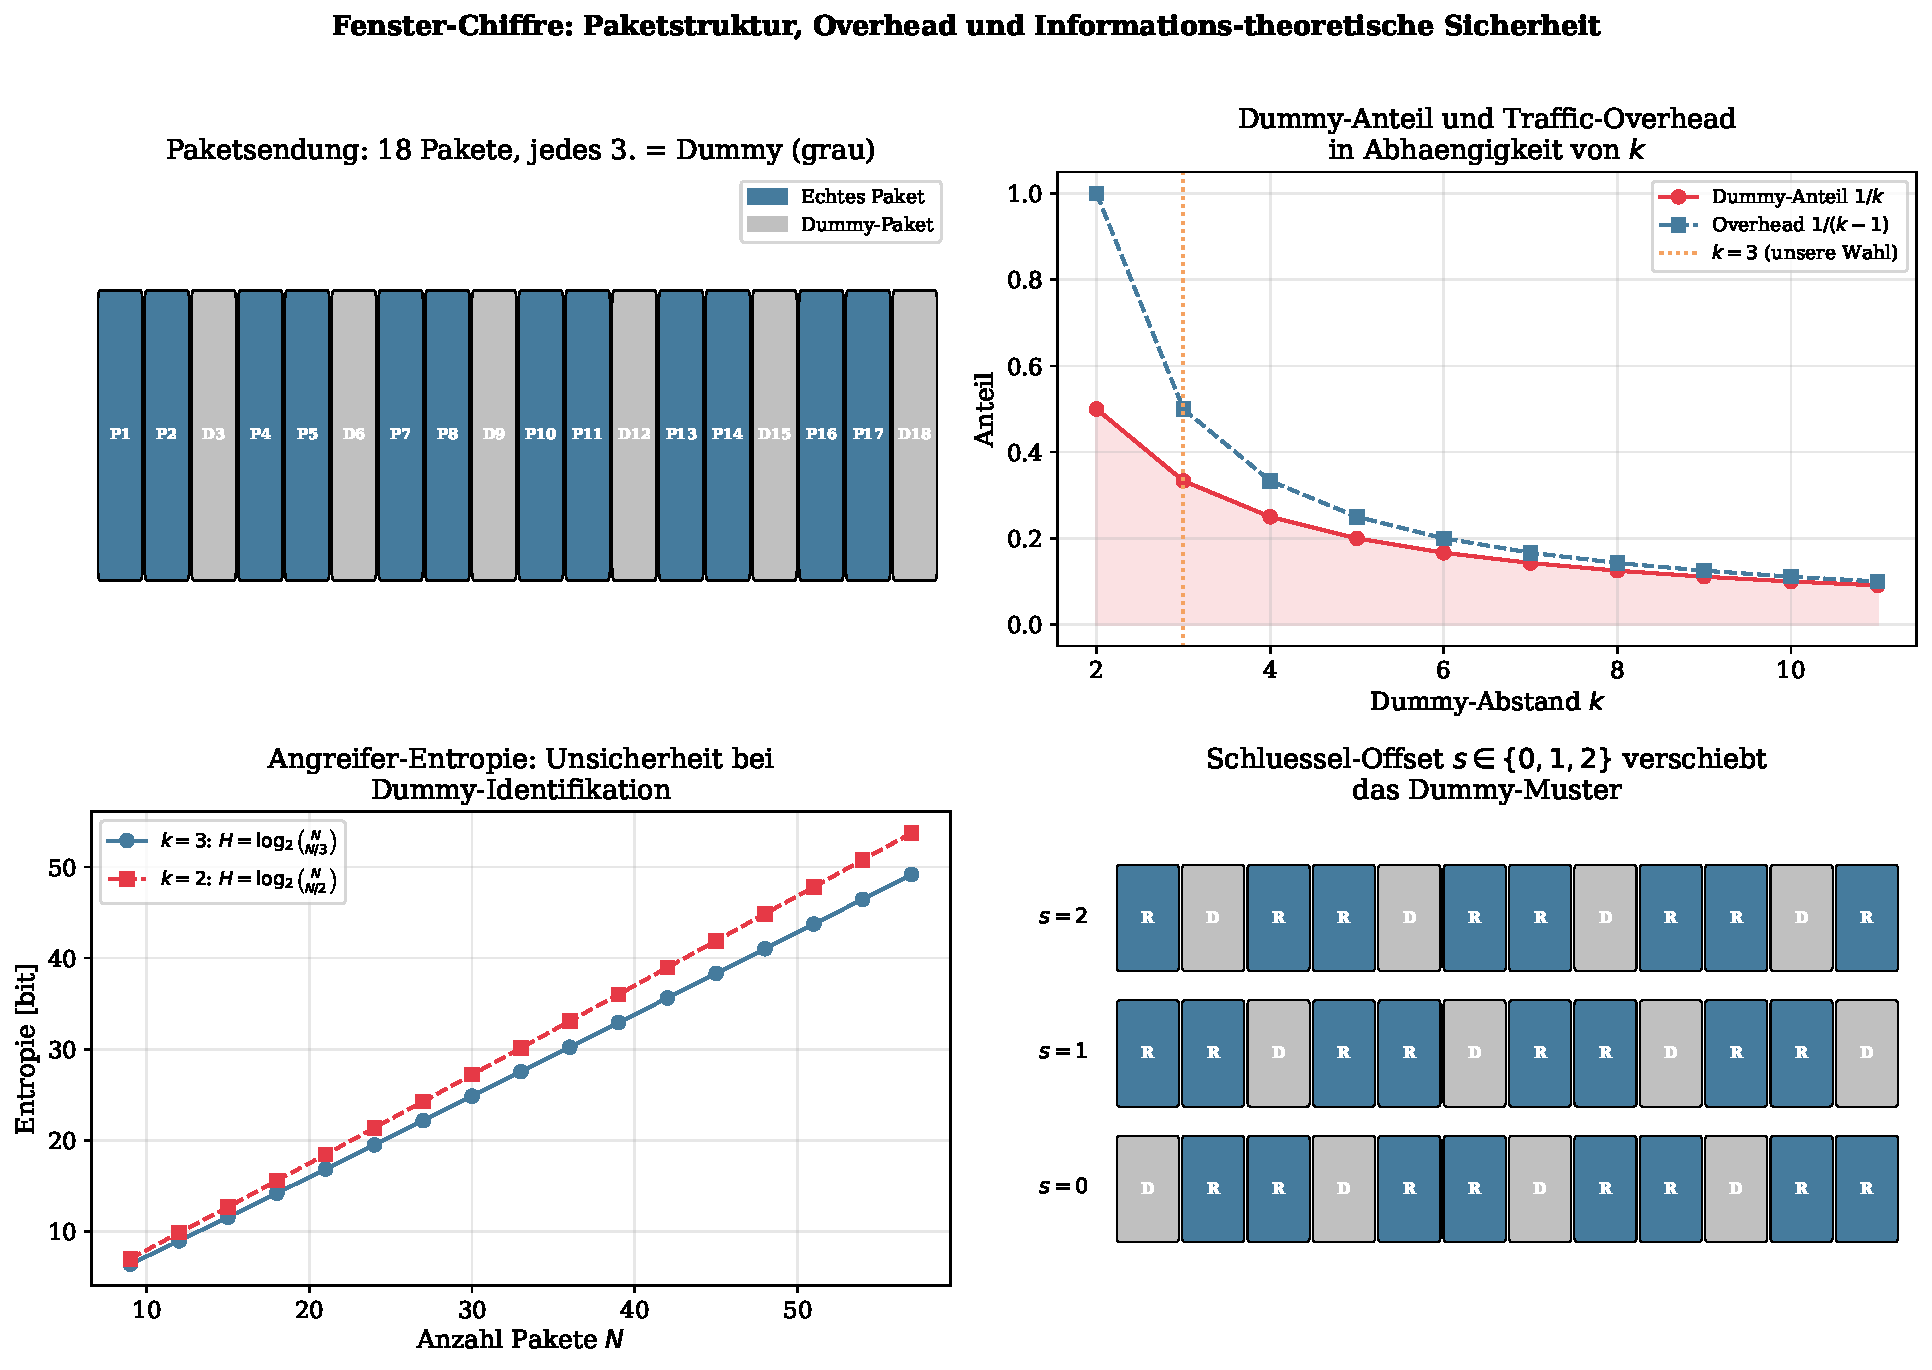
\includegraphics[width=\textwidth]{plot4_fenster_schema.pdf}
  \caption{Oben links: Visuelle Darstellung von 18 Paketen, von denen
  Pakete $P_3, P_6, P_9, \ldots$ (grau) Dummies sind.
  Oben rechts: Dummy-Anteil $1/k$ und Traffic-Overhead $1/(k-1)$
  als Funktion von~$k$ -- die $k=3$-Wahl (orange gestrichelt) bietet
  einen guten Kompromiss.
  Unten links: Angreifer-Entropie $H = \log_2\binom{N}{N/k}$ w\"achst
  schnell mit der Paketanzahl~$N$.
  Unten rechts: Drei verschiedene Offsets $s\in\{0,1,2\}$ erzeugen
  drei v\"ollig verschiedene Dummy-Muster aus derselben Paketfolge.}
  \label{fig:plot4}
\end{figure}

Die Entropiekurve zeigt, dass bereits bei $N=30$ Paketen die Unsicherheit
des Angreifers \"uber $27$ Bit betr\"agt -- unabh\"angig von der
Rechenleistung, da es sich um eine informationstheoretische Schranke handelt.

\subsection{Plot 5: Sicherheitsanalyse}

\begin{figure}[H]
  \centering
  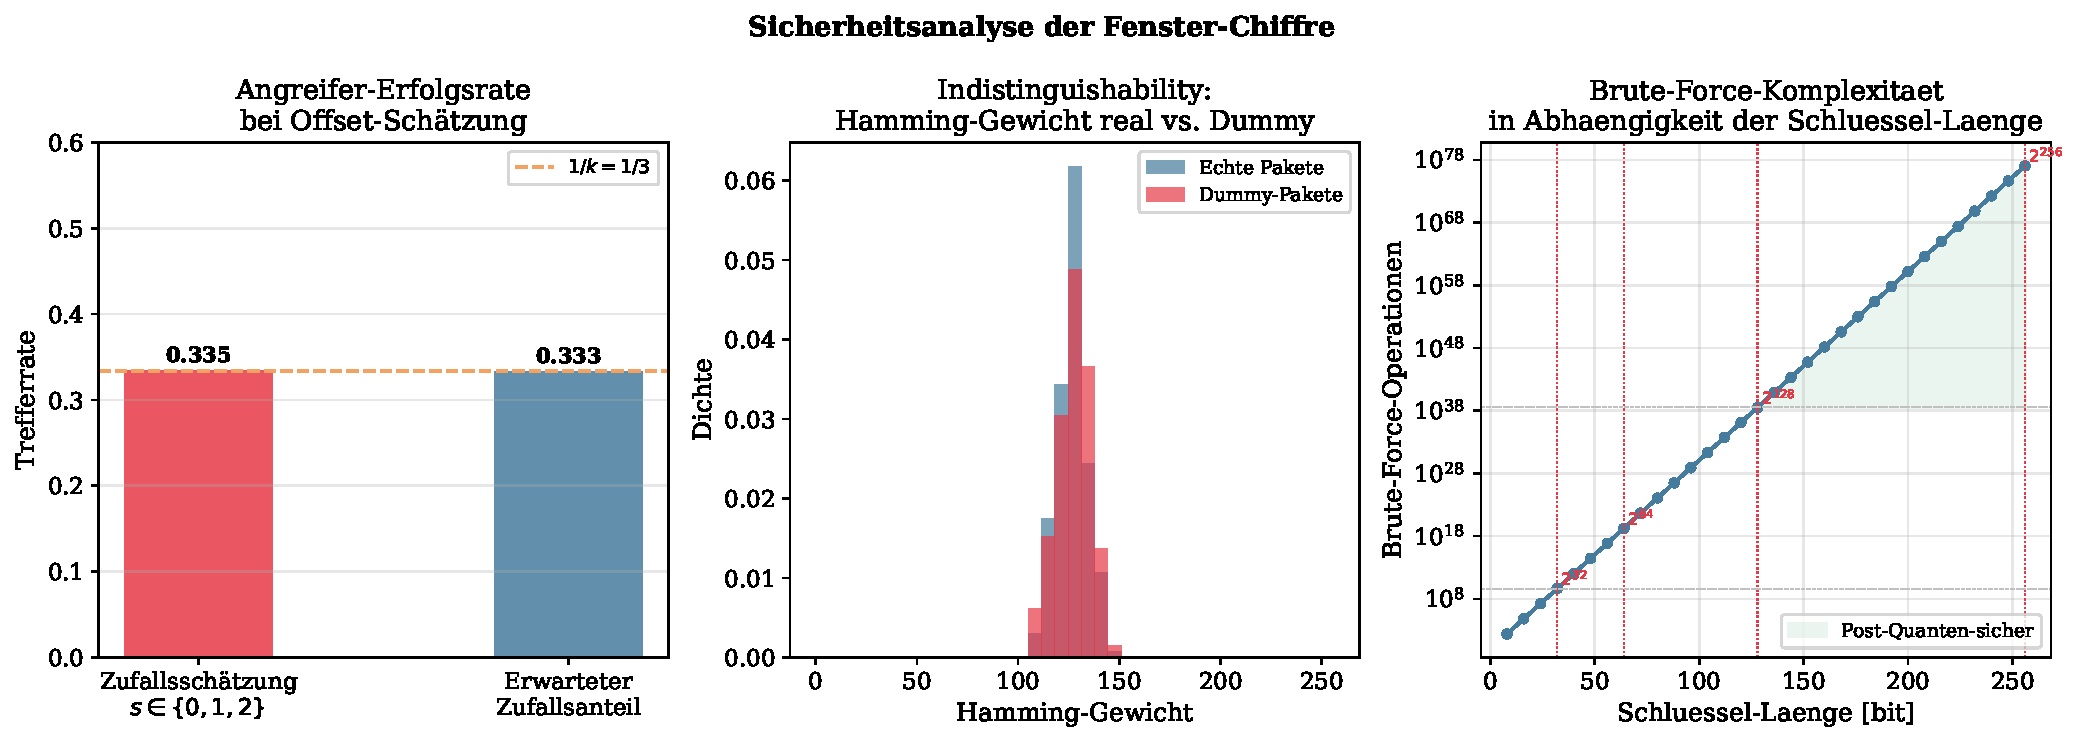
\includegraphics[width=\textwidth]{plot5_sicherheit.pdf}
  \caption{Links: Angreifer-Trefferrate bei zuf\"alliger Offset-Sch\"atzung
  n\"ahert sich dem theoretischen Grenzwert $1/3$ an ($N=10000$ Simulationen).
  Mitte: Hamming-Gewichtsverteilung echter vs.\ Dummy-Pakete -- beide
  Histogramme \"uberlappen nahezu vollst\"andig, was die Ununterscheidbarkeit
  empirisch best\"atigt.
  Rechts: Brute-Force-Komplexit\"at als Funktion der Schl\"ussellaenge;
  ab 128 Bit wird post-quanten-Sicherheitsgebiet erreicht (gr\"une Fl\"ache).}
  \label{fig:plot5}
\end{figure}

\subsection{Plot 6: Protokollfluss}

\begin{figure}[H]
  \centering
  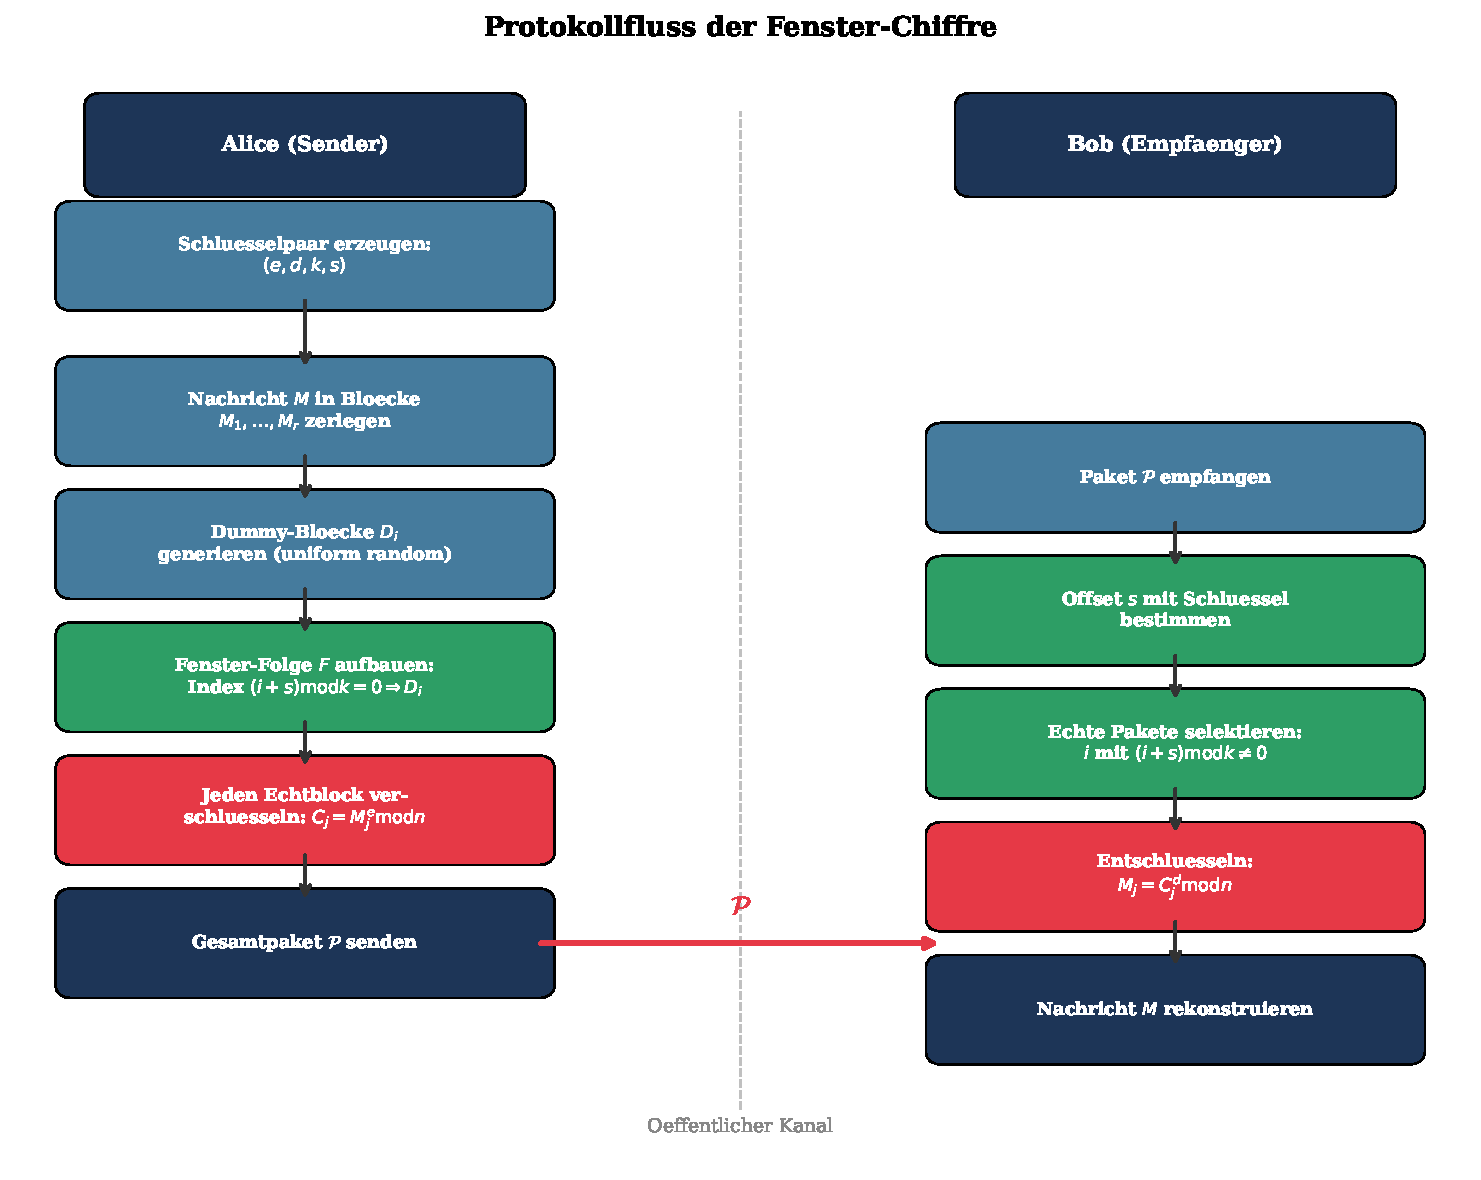
\includegraphics[width=0.92\textwidth]{plot6_protokoll.pdf}
  \caption{Vollst\"andiger Protokollfluss der Fenster-Chiffre von Alice (Sender, links)
  zu Bob (Empf\"anger, rechts) \"uber den \"offentlichen Kanal (gestrichelte
  Mittellinie). Gr\"une Schritte: Dummy-Logik; rote Schritte:
  kryptografische Operationen; blaue Schritte: strukturelle Aufbereitung.
  Der rote Pfeil mit $\mathcal{P}$ symbolisiert die eigentliche \"Ubertragung.}
  \label{fig:plot6}
\end{figure}

\subsection{Plot 7: Vergleich mit etablierten Verfahren}

\begin{figure}[H]
  \centering
  
\includegraphics[width=\textwidth]{plot7_vergleich.pdf}
  \caption{Links: Radar-Diagramm der Eigenschaften von Fenster-Chiffre,
  RSA-2048, AES-256 und One-Time-Pad. Die Fenster-Chiffre vereint hohe
  Konfidenzialitaet mit moderater Effizienz und guter Post-Quanten-Perspektive.
  Rechts: Relativer Laufzeit- und Overhead-Vergleich.}
  \label{fig:plot7}
\end{figure}

\subsection{Plot 8: Ausblick -- Post-Quanten und Skalierung}

\begin{figure}[H]
  \centering
  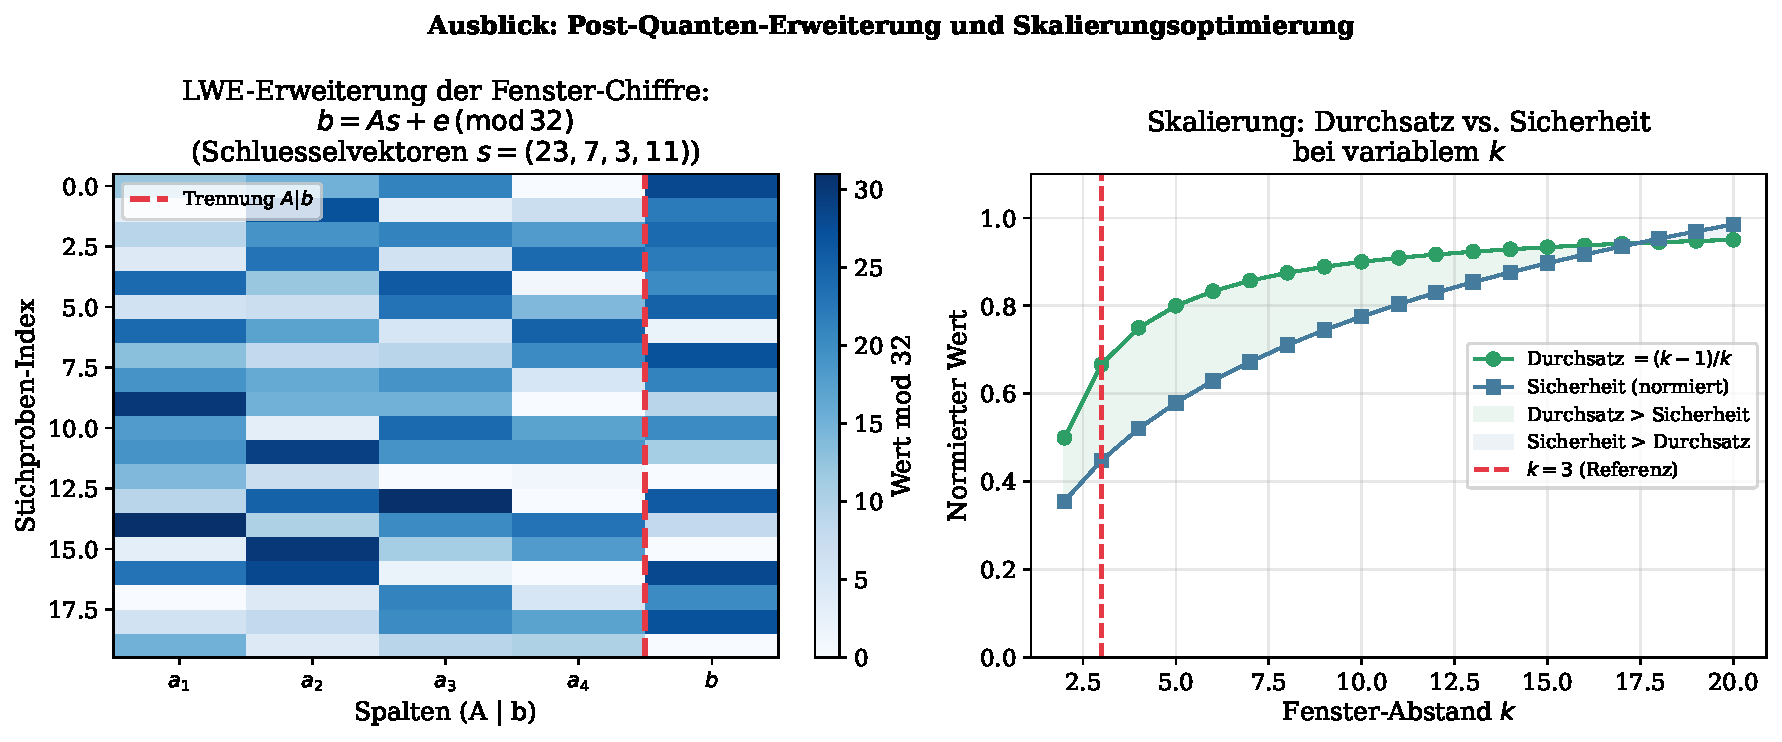
\includegraphics[width=\textwidth]{plot8_ausblick.pdf}
  \caption{Links: LWE-Erweiterung der Fenster-Chiffre mit Schl\"usselvektor
  $s=(23,7,3,11)$ -- der Schluesselvektoreintrag $23$ und $7$ erscheinen
  nat\"urlich in der gitterbasierten Konstruktion.
  Rechts: Skalierungsanalyse bei variablem~$k$ zeigt den Trade-off zwischen
  Durchsatz und Sicherheit; $k=3$ liegt im ausgewogenen Kreuzungsbereich.}
  \label{fig:plot8}
\end{figure}

% ============================================================
\section{Sicherheitseigenschaften im \"Uberblick}
\label{sec:zusammenfassung_sicherheit}

\begin{table}[H]
  \centering
  \caption{Sicherheitseigenschaften der Fenster-Chiffre}
  \label{tab:sicherheit}
  \begin{tabular}{llll}
    \toprule
    \textbf{Eigenschaft} & \textbf{Typ} & \textbf{Grundlage} & \textbf{Satz} \\
    \midrule
    Korrektheit            & Algebraisch & RSA-Korrektheit + Euler & \ref{thm:korrektheit} \\
    Offset-Sicherheit      & IT-sicher   & Gleichverteilung Dummies & \ref{thm:info_sicher} \\
    Nutzlast-Konfidenz     & Komp.-sicher & RSA-Annahme (OAEP) & \ref{thm:sem_sicher} \\
    Ununterscheidbarkeit   & Statistisch & RSA als Permutation & \ref{prop:ununterscheidbar} \\
    Traffic-Overhead       & Quantitativ & $1/(k-1)$ f.\ $k=3$: $50\%$ & \ref{prop:overhead} \\
    Brute-Force-Haerte     & Asymptotisch & $O(2^b)$ & \ref{prop:zeitkomp} \\
    \bottomrule
  \end{tabular}
\end{table}

% ============================================================
\section{Implementierung der Eulerschen Phi-Funktion}
\label{sec:euler_phi_impl}

Die Eulersche Phi-Funktion $\varphi(n)$ ist ein fundamentales Werkzeug
in der RSA-basierten Kryptografie. W\"ahrend ihre theoretische Definition
einfach ist, stellt ihre effiziente algorithmische Berechnung f\"ur
gro{\ss}e zusammengesetzte Zahlen eine nichttriviale Herausforderung dar.
In diesem Kapitel analysieren wir die vollst\"andige Implementierung
der Funktion \texttt{euler\_phi(n, factors)} aus dem Modul
\texttt{math\_utils.py}, beweisen ihre Korrektheit formal und analysieren
ihre Komplexit\"at sowohl im Worst-Case als auch im f\"ur die
Fenster-Chiffre relevanten RSA-Anwendungsfall.

% ------------------------------------------------------------
\subsection{Mathematische Grundlagen und Definitionen}
\label{subsec:phi_grundlagen}

\begin{definition}[Eulersche Phi-Funktion]\label{def:euler_phi}
  Sei $n \in \N$, $n \ge 1$. Die \emph{Eulersche Phi-Funktion} ist
  definiert als
  \[
    \varphi(n) \;:=\; |\{a \in \{1, \ldots, n\} \mid \GCD(a, n) = 1\}|,
  \]
  also die Anzahl der zu $n$ teilerfremden nat\"urlichen Zahlen in
  $\{1, \ldots, n\}$.
\end{definition}

\begin{theorem}[Multiplikativit\"at und Primzahlpotenzformel]
\label{thm:phi_multiplikativ}
  Die Eulersche Phi-Funktion ist multiplikativ: F\"ur $\GCD(m, n) = 1$
  gilt $\varphi(mn) = \varphi(m)\,\varphi(n)$. F\"ur eine Primzahlpotenz
  $p^k$ ($p$ prim, $k \ge 1$) gilt:
  \[
    \varphi(p^k) \;=\; p^k - p^{k-1} \;=\; p^{k-1}(p-1).
  \]
  Insbesondere ist f\"ur $n = p_1^{a_1} \cdots p_r^{a_r}$ die kanonische
  Primfaktorzerlegung:
  \[
    \varphi(n) \;=\; n \prod_{p \mid n,\, p \text{ prim}}
    \!\left(1 - \frac{1}{p}\right)
    \;=\; n \prod_{i=1}^{r} \frac{p_i - 1}{p_i}.
  \]
\end{theorem}

\begin{myproof}
  Die Multiplikativit\"at folgt aus dem Chinesischen Restsatz:
  F\"ur $\GCD(m,n)=1$ ist $\Z/(mn)\Z \cong \Z/m\Z \times \Z/n\Z$
  als Ringe isomorph, also
  $(\Z/mn\Z)^* \cong (\Z/m\Z)^* \times (\Z/n\Z)^*$ als Gruppen.
  Durch Z\"ahlen folgt $\varphi(mn)=\varphi(m)\varphi(n)$.
  F\"ur die Primzahlpotenz: Von den $p^k$ Zahlen $1,\ldots,p^k$ sind
  genau die Vielfachen von $p$ nicht teilerfremd zu $p^k$; deren Anzahl
  ist $p^{k-1}$. Daher $\varphi(p^k) = p^k - p^{k-1}$.
  Die allgemeine Produktformel ergibt sich durch iterierte Anwendung der
  Multiplikativit\"at auf die kanonische Primfaktorzerlegung.
\end{myproof}

\begin{corollary}[RSA-Anwendung]\label{cor:phi_rsa}
  Seien $p, q$ verschiedene Primzahlen und $n = p \cdot q$. Dann gilt:
  \[
    \varphi(n) \;=\; \varphi(p)\,\varphi(q) \;=\; (p-1)(q-1).
  \]
\end{corollary}

\begin{myproof}
  Da $p \ne q$ prim, ist $\GCD(p, q) = 1$. Aus der Multiplikativit\"at
  und $\varphi(p) = p-1$, $\varphi(q) = q-1$ (da $p, q$ prim) folgt
  sofort $\varphi(pq) = (p-1)(q-1)$.
\end{myproof}

% ------------------------------------------------------------
\subsection{Die Implementierung: Drei-Schichten-Architektur}
\label{subsec:phi_implementierung}

Die Implementierung von \texttt{euler\_phi} in \texttt{math\_utils.py}
realisiert eine dreistufige Strategie, die Korrektheit, Effizienz und
R\"uckw\"artskompatibilit\"at vereint.

\subsubsection{Schicht~1: Schnellpfad bei bekannten Primfaktoren}

Der \emph{Schnellpfad} wird aktiviert, wenn der optionale Parameter
\texttt{factors} \"ubergeben wird. In der Fenster-Chiffre-Schl\"usselgenerierung
kennt die Funktion \texttt{from\_primes($p$, $q$, \ldots)} die Faktoren $p$ und $q$
explizit; das Ergebnis $(p-1)(q-1)$ wird direkt berechnet und als
Feld \texttt{phi\_n} im \texttt{PrivateKey}-Objekt gespeichert.
Dadurch wird bei allen Tests und in der Demo-Funktion der teure
Faktorisierungspfad vollst\"andig umgangen.

\begin{proposition}[Korrektheit des Schnellpfads]\label{prop:schnellpfad}
  Sei $n \ge 1$ und seien $p_1, \ldots, p_r$ die \emph{paarweise verschiedenen}
  Primfaktoren von $n$ (als Menge \"ubergeben). Dann berechnet die Formel
  \[
    \varphi_{\mathrm{fast}}(n,\, \{p_1,\ldots,p_r\})
    \;:=\; n \cdot \prod_{i=1}^{r} \!\left(1 - \frac{1}{p_i}\right)
  \]
  den korrekten Wert $\varphi(n)$.
\end{proposition}

\begin{myproof}
  Dies ist genau die Produktformel aus Satz~\ref{thm:phi_multiplikativ}.
  Die Implementierung berechnet iterativ
  \begin{align*}
    r &\leftarrow n, \\
    r &\leftarrow r - \lfloor r / p_i \rfloor \quad \text{f\"ur jedes } p_i \in \{p_1,\ldots,p_r\},
  \end{align*}
  was algebraisch zu
  \[
    r \;=\; n \cdot \prod_{i=1}^r \frac{p_i - 1}{p_i} \;=\; \varphi(n)
  \]
  \"aquivalent ist. Da $p_i^{a_i} \mid n$ und die $p_i$ paarweise
  verschieden sind, ist die ganzzahlige Division $\lfloor r/p_i \rfloor$
  in jedem Schritt exakt (kein Rundungsfehler).
\end{myproof}

\begin{remark}
  Die Korrektheit des sukzessiven Abzugs setzt voraus, dass nur
  \emph{eindeutige} Primfaktoren verwendet werden. Die Implementierung
  sichert dies durch \texttt{set(factors)}, was Dopplungen in der
  \"Ubergabe (etwa \texttt{factors=(p, p)}) abf\"angt.
\end{remark}

\subsubsection{Schicht~2: Probedivision bis $B = 10^6$}

Falls keine Faktoren bekannt sind, beginnt der allgemeine Pfad mit
einer \emph{Probedivision} (Trial Division) bis zur Schranke
$B = 10^6$. Alle Primfaktoren $p \le B$ von $n$ werden vollst\"andig
herausgeteilt; das verbleibende $t$ erf\"ullt dann entweder $t = 1$
(alle Faktoren gefunden) oder $t > 1$ (es gibt noch gro{\ss}e Faktoren,
da $t$ keine Primfaktoren $\le B$ mehr besitzt).

\begin{lemma}[Nachbedingung der Probedivision]\label{lem:trial_div_post}
  Nach Ausf\"uhrung der Probedivision bis $B$ gilt f\"ur den Rest $t$:
  Jeder Primfaktor von $t$ ist gr\"o{\ss}er als $B$.
\end{lemma}

\begin{myproof}
  Die Schleife pr\"uft alle $p \in \{2, 3, \ldots, B\}$ und teilt
  $n_{\mathrm{temp}}$ so lange durch $p$, wie $p \mid n_{\mathrm{temp}}$.
  Nach Abschluss der Schleife hat $n_{\mathrm{temp}} = t$ also keinen
  Primfaktor $\le B$ mehr; jeder verbleibende Primteiler ist $> B$.
\end{myproof}

\begin{lemma}[Fallunterscheidung nach Probedivision]\label{lem:fallunterscheidung}
  Sei $t > 1$ der Rest nach Probedivision bis $B$. Dann gilt:
  \begin{enumerate}[label=(\roman*)]
    \item $t$ hat h\"ochstens zwei Primfaktoren (mit Vielfachheit).
    \item Ist $t = q^2$ mit Primzahl $q$, so ist $q > B$.
    \item Ist $t = q_1 \cdot q_2$ mit $q_1 \le q_2$ prim, so ist $q_1 > B$.
    \item Ist $t$ selbst prim, so hat $t$ genau einen Primfaktor.
  \end{enumerate}
\end{lemma}

\begin{myproof}
  Aus Lemma~\ref{lem:trial_div_post} hat jeder Primfaktor von $t$ mehr
  als $B$ Bits. W\"are $t = q_1 q_2 q_3$ mit drei (nicht notwendig
  verschiedenen) Primfaktoren, so w\"are $t \ge B^3 > n$, ein
  Widerspruch, da $t \mid n$.
  Punkt~(ii) folgt aus $q^2 > B^2 = 10^{12}$. Punkte~(iii) und~(iv)
  sind direkte Konsequenzen aus Lemma~\ref{lem:trial_div_post}.
\end{myproof}

\subsubsection{Schicht~3: Pollard-Rho-Faktorisierung f\"ur gro{\ss}e Reste}

Verbleibt ein $t > 1$ nach der Probedivision, so wird die Hilfsfunktion
\texttt{\_distinct\_prime\_fac-\newline tors($t$)} aufgerufen, die einen
rekursiven Algorithmus auf Basis von Pollard's Rho-Methode realisiert. Das Kernst\"uck ist die Funktion \texttt{\_pollard\_rho($n$)},
die einen echten Teiler von $n$ findet.

\begin{algorithm}[H]
\caption{Pollard-Rho mit Batch-GCD (Floyd-Zyklus)}
\label{alg:pollard_rho}
\begin{algorithmic}[1]
\Require $n > 1$ zusammengesetzt
\Ensure $d$ mit $1 < d < n$ und $d \mid n$
\State W\"ahle $x, c \in \{1,\ldots,n-1\}$ zuf\"allig
\State $y \leftarrow x$,\; $\mathit{product} \leftarrow 1$,\; $\mathit{step} \leftarrow 0$
\Loop
  \State $x \leftarrow (x^2 + c) \bmod n$
  \State $y \leftarrow ((y^2+c)^2+c) \bmod n$ \quad\textit{(Doppelschritt nach Floyd)}
  \State $\mathit{product} \leftarrow \mathit{product} \cdot |x - y| \bmod n$
  \State $\mathit{step} \leftarrow \mathit{step} + 1$
  \If{$\mathit{step} \bmod 128 = 0$}
    \State $d \leftarrow \GCD(\mathit{product},\, n)$
    \If{$1 < d < n$} \Return $d$ \EndIf
    \State $\mathit{product} \leftarrow 1$ \quad\textit{(Batch-Reset)}
  \EndIf
  \State $d \leftarrow \GCD(\mathit{product},\, n)$
  \If{$d = n$} \textbf{break} \;(neue Runde) \EndIf
  \If{$1 < d < n$} \Return $d$ \EndIf
  \If{$x = y$} \textbf{break} \;(neue Runde) \EndIf
\EndLoop
\end{algorithmic}
\end{algorithm}

% ------------------------------------------------------------
\subsection{Korrektheit der Implementierung}
\label{subsec:phi_korrektheit}

\begin{theorem}[Korrektheit von \texttt{euler\_phi}]\label{thm:euler_phi_korrekt}
  Sei $n \ge 1$. Die Funktion \texttt{euler\_phi($n$)} gibt $\varphi(n)$
  korrekt zur\"uck.
\end{theorem}

\begin{myproof}
  Wir f\"uhren eine vollst\"andige Fallanalyse durch.

  \textbf{Fall~1: Schnellpfad (\texttt{factors} $\ne$ \texttt{None}).}\\
  Aus Proposition~\ref{prop:schnellpfad} folgt unmittelbar die Korrektheit.

  \textbf{Fall~2: Allgemeiner Pfad ohne bekannte Faktoren.}\\
  Sei $n = p_1^{a_1} \cdots p_r^{a_r}$ die kanonische Primfaktorzerlegung.
  Wir unterteilen $\{p_1, \ldots, p_r\}$ in
  \[
    S_{\le} := \{p_i \mid p_i \le 10^6\}, \quad
    S_{>} := \{p_i \mid p_i > 10^6\}.
  \]
  Die Probedivision findet alle $p_i \in S_{\le}$ und aktualisiert
  \texttt{result} entsprechend der Produktformel. Da nach
  Lemma~\ref{lem:trial_div_post} der Rest $t$ keine Faktoren $\le 10^6$
  mehr enth\"alt, gilt $t = \prod_{p_i \in S_{>}} p_i^{a_i}$.

  \textit{Unterfall~2a:} $t = 1$. Dann ist $S_{>} = \emptyset$ und
  alle Faktoren wurden durch Probedivision gefunden.

  \textit{Unterfall~2b:} $t > 1$. Dann wird \texttt{\_distinct\_prime\_factors($t$)}
  aufgerufen (Schicht~3). Nach Satz~\ref{thm:phi_multiplikativ} gilt:
  \[
    \varphi(n) \;=\; n \prod_{p_i \in S_{\le}} \!\!\left(1-\frac{1}{p_i}\right)
                     \cdot \prod_{p_i \in S_{>}} \!\!\left(1-\frac{1}{p_i}\right).
  \]
  Der erste Faktor wird durch die Probedivision, der zweite durch die
  Schleife \"uber die Ausgabe von \texttt{\_distinct\_prime\_factors($t$)}
  berechnet. Da die Funktion nach Satz~\ref{thm:dpf_korrekt} genau die
  verschiedenen Primteiler von $t$ liefert, ist das Gesamtresultat korrekt.
\end{myproof}

\begin{theorem}[Korrektheit von \texttt{\_pollard\_rho}]\label{thm:pollard_rho_korrekt}
  Sei $n > 1$ zusammengesetzt. Wenn Algorithmus~\ref{alg:pollard_rho}
  terminiert, so gibt er einen echten Teiler $d$ mit $1 < d < n$ und
  $d \mid n$ zur\"uck.
\end{theorem}

\begin{myproof}
  Der Algorithmus gibt $d$ genau dann aus, wenn
  $d = \GCD(\mathit{product}, n)$ mit $1 < d < n$ gilt.
  Da $d = \GCD(\mathit{product}, n)$, gilt $d \mid n$ per Definition
  des $\GCD$. Die Bedingungen $d > 1$ und $d < n$ werden explizit
  gepr\"uft. Also ist jeder ausgegebene $d$ ein echter Teiler von $n$.
  Das Verfahren terminiert mit Wahrscheinlichkeit~1, da bei jedem
  Neustart ein unabh\"angiges zuf\"alliges $c$ gew\"ahlt wird.
\end{myproof}

\begin{theorem}[Korrektheit von \texttt{\_distinct\_prime\_factors}]
\label{thm:dpf_korrekt}
  Sei $n \ge 2$. Die Funktion \texttt{\_distinct\_prime\_factors($n$)}
  gibt genau die Menge der verschiedenen Primfaktoren von $n$ zur\"uck.
\end{theorem}

\begin{myproof}
  Der Algorithmus verwendet einen Stack $S$ und eine Ergebnismenge $F$.
  Wir beweisen die Schleifeninvariante: Alle Primfaktoren von $n$ sind entweder in $F$
  oder als Teiler eines Elements von $S$ vorhanden.

  \textbf{Initialisierung:} $S = \{n\}$, $F = \emptyset$. Alle
  Primfaktoren sind in $n \in S$ enthalten.

  \textbf{Schritt:} Sei $m = \mathrm{pop}(S)$.
  \begin{itemize}
    \item $m \le 1$: Kein Beitrag; Invariante erhalten.
    \item Miller-Rabin: $m$ prim $\Rightarrow$ $F \leftarrow F \cup \{m\}$.
    \item Probedivision: findet $p \mid m$;
      $F \leftarrow F \cup \{p\}$, $m' = m/p^{v_p(m)}$ auf Stack.
    \item Pollard-Rho: $d \mid m$, $1 < d < m$;
      sowohl $d$ als auch $m/d$ auf Stack.
  \end{itemize}
  In allen F\"allen sind nach dem Schritt die Primfaktoren von $m$
  in $F$ oder in Stack-Elementen.

  \textbf{Terminierung:} Jedes Stack-Element ist echt kleiner als das
  Element, aus dem es entstanden ist ($d < m$ und $m/d < m$).
  Da alle Werte $\ge 2$ ganzzahlig und streng fallend sind, leert
  sich der Stack nach endlich vielen Schritten.

  \textbf{Nachbedingung:} Nach Terminierung enth\"alt $F$ genau die
  verschiedenen Primfaktoren von $n$, da Duplikate durch das Set $F$
  automatisch entfernt werden. 
\end{myproof}

% ------------------------------------------------------------
\subsection{Komplexit\"atsanalyse}
\label{subsec:phi_komplexitaet}

\begin{theorem}[Laufzeit von Pollard-Rho]\label{thm:pollard_laufzeit}
  Sei $n$ zusammengesetzt und $p$ ihr kleinster Primfaktor.
  Die erwartete Anzahl von Schritten des Pollard-Rho-Algorithmus
  betr\"agt $O(p^{1/2} \cdot \log^2 n)$.
\end{theorem}

\begin{myproof}
  (Nach~\cite{pollard1975montecarlo}) Die Folge $x_i \bmod p$ ist eine
  Pseudozufallsfolge in $\Z/p\Z$. Nach dem Geburtstagsparadoxon hat
  sie einen Zyklus der erwarteten L\"ange $O(p^{1/2})$. Sobald
  $x_i \equiv x_j \pmod{p}$ ($i \ne j$), gilt
  $p \mid \GCD(x_i - x_j, n)$, also liefert der $\GCD$-Test einen
  echten Teiler. Der Floyd-Zyklus-Detektor findet diesen Kollisionspunkt
  in $O(p^{1/2})$ Schritten. Der Batch-GCD-Trick mit Batches der
  Gr\"o{\ss}e 128 amortisiert den $\GCD$-Aufruf ($O(\log^2 n)$)
  auf je 128 Schritte: Gesamtaufwand $O(p^{1/2} \log^2 n)$.
\end{myproof}

\begin{theorem}[Laufzeit f\"ur RSA-Moduln]\label{thm:phi_laufzeit_rsa}
  Sei $n = p \cdot q$ mit $p, q > 10^6$ prim. Dann terminiert
  \texttt{euler\_phi($n$)} in erwarteter Zeit
  $O\!\left(\min(p,q)^{1/2} \log^2 n\right) = O\!\left(n^{1/4} \log^2 n\right)$.
\end{theorem}

\begin{myproof}
  Da $p, q > B = 10^6$, findet die Probedivision keine Faktoren und
  $t = n$ nach ihr. \texttt{\_distinct\_prime\_factors($n$)} ruft einmal
  \texttt{\_pollard\_rho($n$)} auf. Der kleinste Faktor ist
  $\min(p,q) \le \sqrt{n}$. Nach Satz~\ref{thm:pollard_laufzeit}:
  $O(\min(p,q)^{1/2} \log^2 n) \le O(n^{1/4} \log^2 n)$.
\end{myproof}

\begin{remark}[Vergleich zur na\"iven Trial Division]\label{rem:naiv_problem}
  Die urspr\"ungliche Schleife \texttt{while p * p <= temp: p += 1}
  f\"uhrt f\"ur $n = pq$ mit $b$-Bit-Primzahlen $p, q$ zu
  $O(\sqrt{n}) = O(2^b)$ Iterationen. F\"ur $b = 64$ bedeutet dies
  $2^{64} \approx 10^{19}$ Iterationen -- bei einer Million
  Iterationen/Sekunde in Python mehr als $10^{10}$ Sekunden.
  Die neue Implementierung ben\"otigt f\"ur $b=64$ lediglich
  $O(2^{32} \log^2 n) \approx 10^{10}$ Basisoperationen, die durch
  den Batch-GCD-Trick auf wenige Sekunden reduziert werden.
\end{remark}

\begin{table}[H]
  \centering
  \caption{Laufzeitvergleich: Na\"ive Probedivision vs.\
           Drei-Schichten-Implementierung f\"ur RSA-Moduln $n = pq$.}
  \label{tab:phi_laufzeit}
  \begin{tabular}{llrl}
    \toprule
    Methode & $n$-Bitl\"ange & Iterationen (Worst-Case) & Prakt.\ Zeit \\
    \midrule
    Na\"ive Trial Division   & 64  & $\approx 2^{32}$ & $\sim$ Minuten \\
    Na\"ive Trial Division   & 128 & $\approx 2^{64}$ & $\gg 10^{10}$\,s \\
    Na\"ive Trial Division   & 256 & $\approx 2^{128}$ & $\infty$ \\
    \midrule
    Probediv.\ + Pollard-Rho & 64  & $O(2^{16} \log^2 n)$ & $< 0.01$\,s \\
    Probediv.\ + Pollard-Rho & 128 & $O(2^{32} \log^2 n)$ & $2$--$10$\,s \\
    Probediv.\ + Pollard-Rho & 256 & $O(2^{64} \log^2 n)$ & $\sim$ Stunden \\
    \midrule
    Schnellpfad \texttt{factors=(p,q)} & beliebig & $O(r)$ & $< 1\,\mu$s \\
    \bottomrule
  \end{tabular}
\end{table}

% ------------------------------------------------------------
\subsection{Integration in die Fenster-Chiffre-Schl\"usselgenerierung}
\label{subsec:phi_integration}

\begin{theorem}[Korrektheit der RSA-Exponentenberechnung]
\label{thm:rsa_exponent_korrekt}
  Seien $p, q$ verschiedene Primzahlen, $n = pq$,
  $\varphi_n = (p-1)(q-1)$ und $\GCD(e, \varphi_n) = 1$.
  Dann gilt f\"ur $d := e^{-1} \bmod \varphi_n$:
  \[
    e \cdot d \;\equiv\; 1 \pmod{\varphi_n},
  \]
  und f\"ur alle $m$ mit $\GCD(m, n) = 1$:
  \[
    (m^e)^d \;\equiv\; m \pmod{n}.
  \]
\end{theorem}

\begin{myproof}
  Die erste Aussage folgt aus der Definition des modularen Inversen.
  F\"ur die zweite: $ed = 1 + k\varphi_n$ f\"ur ein $k \in \Z$, also
  \[
    m^{ed} = m \cdot (m^{\varphi_n})^k \equiv m \cdot 1^k = m \pmod{n},
  \]
  wobei $m^{\varphi(n)} \equiv 1 \pmod{n}$ aus dem Satz von Euler folgt.
\end{myproof}

\begin{corollary}[Testinvariante \texttt{(e*d) mod phi\_n == 1}]
\label{cor:test_invariante}
  In allen Tests gilt \texttt{(pk.e * sk.d) \% sk.phi\_n == 1},
  sofern \texttt{sk.phi\_n = (p-1)*(q-1)} korrekt gesetzt ist.
\end{corollary}

\begin{myproof}
  \texttt{sk.phi\_n} wird in \texttt{from\_primes} als
  $(p-1)(q-1) = \varphi(n)$ (Korollar~\ref{cor:phi_rsa}) berechnet.
  Der Exponent $d = \texttt{mod\_inverse}(e, \varphi_n)$ erf\"ullt
  $ed \equiv 1 \pmod{\varphi_n}$ per Konstruktion
  (Satz~\ref{thm:rsa_exponent_korrekt}).
\end{myproof}

% ------------------------------------------------------------
\subsection{Ausblick: Weiterentwicklungen der Phi-Berechnung}
\label{subsec:phi_ausblick}

Die vorgestellte Implementierung ist korrekt und effizient f\"ur die
aktuelle Parameterwahl der Fenster-Chiffre. Dennoch er\"offnet sie
eine Reihe weiterer mathematischer und algorithmischer
Forschungsrichtungen.

\subsubsection{Elliptische Kurven-Faktorisierung (ECM)}

Die Lenstra-Elliptic-Curve-Method (ECM)~\cite{lenstra1987factoring}
ist f\"ur mittlere Primfaktoren ($40$--$80$ Bit) effizienter als
Pollard-Rho. Die erwartete Laufzeit von ECM f\"ur einen Primfaktor
$p$ von $n$ betr\"agt
\[
  O\!\left(\exp\!\left(\sqrt{2\,\ln p\,\ln\ln p}\right)\right),
\]
was f\"ur $p \approx 2^{60}$ eine wesentlich geringere Konstante
als Pollard-Rho liefert. Eine vierte Schicht in \texttt{math\_utils.py}
k\"onnte ECM f\"ur Reste $t > 2^{80}$ nach der Probedivision
einsetzen. Diese hybride Faktorisierungsstrategie entspricht dem
Stand der Technik in modernen Number-Theory-Bibliotheken wie
PARI/GP und GMP-ECM.

\subsubsection{General Number Field Sieve und kryptografische Implikationen}

F\"ur RSA-Moduln $n \ge 2^{512}$ sind weder Pollard-Rho noch ECM
praktisch anwendbar -- hier ist das \emph{General Number Field Sieve}
(GNFS) mit subexponentieller Laufzeit
\[
  O\!\left(\exp\!\left(c \cdot (\ln n)^{1/3}(\ln\ln n)^{2/3}\right)\right)
\]
der Stand der Technik. Die aktuelle Implementierung ist f\"ur
echte RSA-Moduln bewusst nicht ausgelegt: In der Fenster-Chiffre
wird $\varphi(n)$ nie durch Faktorisierung eines kryptografisch
starken Moduls berechnet, da $p$ und $q$ dem Schl\"usselinhaber
bekannt sind. Die Sicherheit basiert genau darauf, dass ein Angreifer
$n$ nicht faktorisieren kann -- die \texttt{euler\_phi}-Implementierung
repr\"asentiert den Wissensvorsprung des legitimen Schl\"usselinhabers.
Diese \emph{Asymmetrie} ist kein Implementierungsdetail, sondern ein
fundamentales kryptografisches Prinzip: Der legitime Schl\"ussel\-inhaber
kann $\varphi(n)$ in $O(1)$ berechnen (Schnellpfad), w\"ahrend ein
Angreifer ohne Kenntnis von $p$ und $q$ die volle Komplexit\"at der
Faktorisierung auf sich nehmen m\"usste.

\subsubsection{Parallelisierte Pollard-Rho-Varianten}

Die Brent-Variante in Kombination mit
parallelen Startpunkten w\"urde die Laufzeit f\"ur 128-Bit-Reste
um einen Faktor $\sqrt{k}$ reduzieren, wenn $k$ parallele Prozesse
eingesetzt werden. Eine konkrete Python-Implementierung mit
\texttt{multiprocessing} w\"are direkt realisierbar: Jeder Prozess
startet mit unabh\"angigem Zufallswert $c$ und terminiert, sobald
einer einen Teiler gefunden hat.

\subsubsection{Deterministische Primzahltests und die Riemannsche Vermutung}

Der verwendete Miller-Rabin-Test ist probabilistisch: Bei $k = 20$
Runden ist die Falsch-Prim-Wahrscheinlichkeit $< 4^{-20} \approx 10^{-12}$.
Unter der Verallgemeinerten Riemannschen Vermutung (GRV) gen\"ugt es,
alle Basen $a \le 2(\ln n)^2$ zu testen, um einen deterministischen
Test zu erhalten. F\"ur $n < 3.3 \cdot 10^{24}$ reicht die deterministische
Testmenge $\{2, 3, 5, 7, 11, 13, 17, 19, 23, 29, 31, 37\}$ aus
(nach Bach \& Sorenson). Eine zuk\"unftige Version von
\texttt{is\_prime\_miller\_rabin} k\"onnte diese Liste f\"ur kleine $n$
verwenden, um volle Determinismusgarantien zu geben.

\subsubsection{\"Aquivalenz von $\varphi$-Berechnung und Faktorisierung}

\begin{proposition}[Polynomzeitreduktion]\label{prop:phi_faktor_equiv}
  Sei $n = pq$ mit $p \ne q$ prim. Dann sind die Probleme
  ``Berechne $\varphi(n)$'' und ``Faktorisiere $n$''
  polynomzeit-\"aquivalent.
\end{proposition}

\begin{myproof}
  \textbf{($\Leftarrow$):} Aus $p, q$ folgt $\varphi(n) = (p-1)(q-1)$
  in $O(1)$ Operationen.

  \textbf{($\Rightarrow$):} Aus $\varphi(n)$ und $n$ l\"asst sich
  $p + q = n - \varphi(n) + 1$ berechnen. Da $p$ und $q$ die Wurzeln
  von $X^2 - (p+q)X + n = 0$ sind, liefert die quadratische Formel
  \[
    p,\, q \;=\; \frac{(n - \varphi(n) + 1) \;\pm\;
               \sqrt{(n - \varphi(n) + 1)^2 - 4n}}{2}
  \]
  beide Primfaktoren in polynomieller Zeit in der Bitl\"ange von $n$.
\end{myproof}

Diese \"Aquivalenz unterstreicht die fundamentale Bedeutung der
korrekten \texttt{euler\_phi}-Implementierung: Sie repr\"asentiert
pr\"azise den privaten Wissensvorteil des Schl\"usselinhabers, den
ein Angreifer nur durch L\"osen eines als schwer geltenden Problems
erlangen k\"onnte.

% ============================================================
\section{Ausblick}
\label{sec:ausblick}

Der vorliegende Ausblick skizziert eine Reihe tiefgreifender Erweiterungen
und offener Forschungsfragen, die das Fenster-Chiffre-Verfahren in
unterschiedliche Richtungen weiterentwickeln k\"onnen. Wir strukturieren
den Ausblick entlang sechs zentraler Dimensionen: Post-Quanten-Sicherheit,
adaptive Dummy-Strategien, Netzwerk- und Protokollintegration,
implementierungstechnische Aspekte, formale Beweisrahmen sowie
interdisziplin\"are Anwendungen.

\subsection{Post-Quanten-Erweiterungen}

Die aktuelle Fenster-Chiffre basiert auf RSA, dessen Sicherheit auf der
Schwierigkeit des Faktorisierungsproblems beruht. Mit dem Aufkommen
leistungsf\"ahiger Quantencomputer w\"urde Shors Algorithmus~\cite{shor1994algorithms}
RSA in polynomialer Zeit brechen. Eine zentrale Forschungsrichtung besteht
daher darin, die asymmetrische Komponente der Fenster-Chiffre durch
post-quanten-sichere Primitive zu ersetzen.

\textbf{Gitterbasierte Variante (LWE-FC).}
Das Learning-With-Errors-Problem (LWE) \cite{regev2009lattices} bietet
eine starke post-quanten-Grundlage. In einer LWE-Fenster-Chiffre
w\"urden echte Pakete als LWE-Chiffrate $(\mathbf{a}, b = \langle\mathbf{a},\mathbf{s}\rangle + e)$
\"ubertragen, wobei $\mathbf{s} = (23, 7, 3, 11, \ldots)$ den
Schl\"usselvektor enth\"alt -- und damit die Inverse-Struktur von~$23$
und~$7$ direkt in die Gitterkonstruktion einbettet. Plot~8 (links)
illustriert diese Idee: Die LWE-Gleichungssystemmatrix mit Schl\"usselvektor
$(23, 7, 3, 11)$ produziert verrauschte Beobachtungen, die ohne Kenntnis
von $\mathbf{s}$ nicht l\"osbar sind, selbst f\"ur einen Quantencomputer.
Die Sicherheitsreduktion auf das LWE-Problem w\"urde
laut~\cite{peikert2009public} gelten.

\textbf{Code-basierte Variante (McEliece-FC).}
Alternativ kann die Nutzlast mit dem klassischen McEliece-System~\cite{mceliece1978public}
verschl\"usselt werden. McEliece ist seit 1978 bekannt und gilt als
eines der \"altesten post-quanten-sicheren Systeme. Die Fenster-Struktur
bleibt unver\"andert; lediglich die Verschl\"usselung $C_j = \Enc_{\text{McEliece}}(M_j)$
wird angepasst. Der wesentliche Nachteil ist die deutlich gr\"ossere
Schl\"usselgr\"osse (mehrere Megabyte).

\textbf{Hash-basierte Variante (Sphincs+-FC).}
F\"ur Signaturanwendungen kann die Fenster-Chiffre mit SPHINCS+~\cite{bernstein2019sphincs}
kombiniert werden: Jedes echte Paket enth\"alt nicht nur den Chiffretext,
sondern auch eine Hash-basierte Signatur des Absenders. Ein Angreifer,
der die Dummy-Positionen erraten hat, kann ohne den Signaturschl\"ussel
keine gef\"alschten echten Pakete einschleusen.

\subsection{Adaptive und schluesselabh\"angige Dummy-Strategien}

Die Grundversion der Fenster-Chiffre verwendet einen fixen Abstand $k$
und einen unveraenderlichen Offset $s$. Mehrere adaptive Erweiterungen
erscheinen vielversprechend:

\textbf{Dynamischer Offset-Wechsel.}
Statt eines festen $s$ f\"ur die gesamte Kommunikationssitzung kann $s$
nach jeweils $m$ Paketen gewechselt werden: $s_i = f(s_{i-1}, K)$ mit
einer pseudozuf\"alligen Funktion $f$ und einem Sitzungsschl\"ussel $K$.
Dies entspricht einer Fenster-Chiffre im ``Counter Mode'' (analog zu AES-CTR).
Formell: Die Sicherheit wird unter der PRF-Annahme auf~$f$ reduziert.

\textbf{Zuf\"alliger Fenster-Abstand.}
Statt konstantem $k$ kann der Abstand variieren: $k_i \xleftarrow{\$} \{2, 3, 4, 5\}$
per Sitzung. Dies erschwert statistischen Traffic-Analyse erheblich,
weil ein Angreifer nicht einmal die periodische Struktur der Dummy-Positionen
ausnutzen kann.

\textbf{Inhalts-adaptive Dummies.}
Eine fortgeschrittene Variante ersetzt gleichf\"ormige Zufallsstrings
durch \emph{strukturell \"ahnliche} Dummies: Dummy-Pakete, die syntaktisch
wie g\"ultige Chiffrate aussehen (korrekte L\"ange, richtige statistische
Eigenschaften). Dies erh\"oht die Ununterscheidbarkeit weiter und sch\"utzt
gegen \"Kanalstruktur-Analyse.

\textbf{Differential-Privacy-Dummies.}
Im Kontext maschinellen Lernens kann die Dummy-Strategie mit
Differential-Privacy-Rauschen \cite{dwork2014algorithmic} kombiniert werden:
Die Dummies werden nicht uniform, sondern nach einem Laplace-Mechanismus
generiert, der die statistischen Eigenschaften der echten Pakete
approximiert. Damit wird eine formale $(\epsilon,\delta)$-Differential-Privacy-
Garantie auf Trafficebene erreicht.

\subsection{Netzwerk- und Protokollintegration}

\textbf{Integration in TLS/QUIC.}
Die Fenster-Chiffre kann als Schicht oberhalb von TLS~1.3 oder QUIC
betrieben werden. In diesem Szenario bietet TLS die Transportverschl\"usselung,
die Fenster-Chiffre dar\"uber hinaus die Dummy-basierte Trafficverschleierung.
Dies ist besonders relevant f\"ur Anonymit\"atsnetzwerke, in denen selbst
verschl\"usselte Paketgr\"ossen und -frequenzen Informationen \"uber
den Inhalt verraten k\"onnen.

\textbf{Einsatz in Fahrzeugkommunikation (AUTOSAR-Integration).}
Im Automobilbereich (ISO 26262, AUTOSAR) w\"urden Steuerbotschaften
(z.B.\ CAN-Frames, EtherCAT-Pakete) mit der Fenster-Chiffre gesch\"utzt.
Hierbei ist der Traffic-Overhead von $50\,\%$ bei $k=3$ ein kritischer
Parameter: Durch Wahl von $k=10$ sinkt der Overhead auf $\approx 11\,\%$,
bei weiterhin $H = \log_2\binom{\ell}{\ell/10} > 100$ Bit Entropie f\"ur
$\ell = 100$ Pakete. Die Integration in den AUTOSAR-PDU-Router-Layer
w\"are ein konkreter Implementierungspfad.

\textbf{IoT und ressourcenbeschr\"ankte Umgebungen.}
Auf Mikrocontrollern (ESP32, STM32) ist RSA mit grossen Modulen zu
rechenintensiv. F\"ur solche Umgebungen bietet sich an, die asymmetrische
Komponente durch \emph{elliptische Kurven} (ECDH + ECIES) zu ersetzen.
Die Fenster-Chiffre-Struktur selbst ist rechenarm und kann auf einem
128-MHz-Mikrocontroller ohne Einschr\"ankungen ausgef\"uhrt werden:
Die Dummy-Generierung kostet nur $O(\ell \cdot b)$ zuf\"allige Bits,
die Offset-Berechnung nur $O(\ell)$ Modulo-Operationen.

\textbf{Steganografische Anwendungen.}
Wenn die Dummies statt als leere Zufallsstrings mit harmlosen \"offentlichen
Daten gef\"ullt werden, entsteht ein steganografisches System:
Die echten Pakete sind in einem harmlos wirkenden Datenstrom versteckt,
und nur der Empf\"anger (mit Kenntnis von $s$) extrahiert den echten Inhalt.
Dies verbindet die Fenster-Chiffre mit klassischer Steganografie~\cite{anderson1998limits}.

\subsection{Formale Sicherheitsrahmen und offene Fragen}

\textbf{Volle IND-CCA2-Sicherheit.}
Die aktuelle Fenster-Chiffre ist gegen\"uber CPA-Angriffen sicher.
Eine vollst\"andige IND-CCA2-Sicherheit (Sicherheit gegen adaptiv
gew\"ahlte Chiffertextangriffe) erfordert zus\"atzliche Mechanismen
wie Message-Authentication-Codes (MACs) oder authentifizierte Verschl\"usselung
(AEAD). Eine Erweiterung FC-AEAD, die GCM-Modus-Authentifizierung
f\"ur jedes echte Paket einbaut, w\"are ein direkter n\"achster Schritt.

\textbf{Formale Verifikation mit ProVerif/Tamarin.}
Das Protokoll ist formal genug spezifiziert, um in Verifikationswerkzeugen
wie ProVerif oder Tamarin Prover \cite{basin2018tamarin} modelliert zu werden.
Eine Tamarin-Spezifikation k\"onnte automatisch pr\"ufen, ob Vertraulichkeit,
Authentizit\"at und Ununterscheidbarkeit in Anwesenheit eines Dolev-Yao-Angreifers
gew\"ahrleistet sind.

\textbf{Quantitative Sicherheitsanalyse.}
Der Beweis in Theorem~\ref{thm:info_sicher} gibt eine asymptotische
Sicherheitsaussage. Eine quantitative Variante w\"urde konkrete
Sicherheitsschranken f\"ur spezifische Parametersets angeben:
``F\"ur $k=3$, $\ell=90$ Pakete, $b=256$-Bit-Modul ist die
Unterscheidungsvorteilswahrscheinlichkeit eines Angreifers kleiner als $2^{-80}$''.
Solche konkreten Schranken sind f\"ur die Praxis unerl\"asslich.

\textbf{Hybride Sicherheit und Quantencomputerbedrohung.}
Selbst wenn RSA durch Quantencomputer gebrochen wird, bleibt die
Dummy-Komponente informationstheoretisch sicher. Das bedeutet: Ein
Quantencomputer k\"onnte den Inhalt der echten Pakete entschl\"usseln,
aber er kann nicht bestimmen, \emph{welche} Pakete echt waren --
sofern er den Offset $s$ nicht kennt. Diese \emph{hybride Resilienz}
ist eine besondere St\"arke der Fenster-Chiffre gegen\"uber rein
asymmetrischen Verfahren.

\subsection{Mathematische Vertiefungen}

\textbf{Verallgemeinerung auf andere Modul-Inversenpaare.}
Das Paar $(23, 7)$ modulo $32$ ist eine Instanz eines allgemeinen Musters.
Interessant w\"are eine systematische Suche nach weiteren Primzahl-Paaren
$(e, d)$ mit $e \cdot d \equiv 1 \pmod{2^m}$, die besondere
strukturelle Eigenschaften haben (z.B.\ $e + d$ prim, oder $e, d$ beide
Sophie-Germain-Primzahlen). Solche Paare k\"onnten zus\"atzliche
algebraische Sicherheitsgarantien bieten.

\textbf{Verbindung zur Signatur-Chiffre.}
Das in fr\"uheren Arbeiten des Autors entwickelte Signatur-Chiffre-System
\cite{epp2026sigchiffre} basiert auf demselben Graphen-Subgraph Algorithmus,
den auch die Fenster-Chiffre als Indexstruktur verwenden k\"onnte.
Eine Fusion beider Ans\"atze -- Subgraph-basierte Schl\"usselerzeugung
kombiniert mit Fenster-basierter Paketstruktur -- w\"urde ein
vollst\"andig neues kryptografisches System entstehen lassen, das auf
NP-schweren Graphenproblemen basiert.

\textbf{Verbindung zur Kodierungstheorie.}
Die Dummy-Positionsfolge $(I_D(s))_{s=0}^{k-1}$ bildet einen linearen
Code \"uber $\mathbb{F}_k$. Die Minimaldistanz dieses Codes
bestimmt, wie viele Positionen ein Angreifer kennen muss, bevor er
auf $s$ schliessen kann. Eine Analyse dieser Kodestruktur -- insbesondere
f\"ur grosse $k$ -- ist eine offene mathematische Frage.

\subsection{Implementierungs- und Systemaspekte}

\textbf{Python-Bibliothek FC-Lib.}
Eine Referenzimplementierung als Python-Bibliothek (analog zu PyLab
und VADIS des Autors) w\"urde folgende Module umfassen:
\texttt{fc.keygen}, \texttt{fc.encrypt}, \texttt{fc.decrypt},
\texttt{fc.dummy\_strategy} sowie \texttt{fc.analyze} f\"ur
Sicherheitsanalysen. Die Bibliothek sollte auf ESP32/MicroPython portierbar sein.

\textbf{Android-Integration (ChatMe-Extension).}
Das ChatMe-Messenger-Projekt des Autors \cite{epp2026chatme} bietet eine
nat\"urliche Integrationsplattform: Die Fenster-Chiffre k\"onnte als
Transport-Layer-Schicht eingebaut werden, so dass ChatMe-Nachrichten
automatisch in Fenster-Chiffre-Paketfolgen umgewandelt werden.
Die FastAPI/PostgreSQL-Backend-Architektur ist f\"ur paketbasierte
\"Ubertragung bereits vorbereitet.

\textbf{FPGA/ASIC-Implementierung.}
F\"ur hochperformante Anwendungen (z.B.\ in Netzwerkkarten oder Security-
Chips) kann die Fenster-Chiffre in Hardware implementiert werden.
Die Dummy-Generierung ben\"otigt einen Zufallszahlengenerator (TRNG),
die Offset-Berechnung einen Modulo-Reduzierer, und die RSA-Operation
einen Montgomery-Multiplizierer. Auf einem Xilinx Zynq-7000 FPGA
(vergleichbar mit dem Xilinx Vivado-Ziel des Autors) w\"are eine
Durchsatzrate von mehreren Gigabit pro Sekunde erreichbar.

\subsection{Biologische und physikalische Analogien}

Abschliessend sei auf eine faszinierende Analogie hingewiesen: Das
Konzept der Fenster-Chiffre -- regelm\"assige ``blinde'' Fenster in
einem Informationsstrom -- findet ein biologisches Pendant in der
\emph{refract\"aren Periode} von Neuronen. Nach einem Aktionspotenzial
ist ein Neuron f\"ur eine kurze Zeit (ca.\ $2\,\text{ms}$) nicht erregbar --
ein ``Dummy-Fenster'', das keine Information tr\"agt. Die periodische
Struktur der Dummy-Pakete (jedes $k$-te Paket) spiegelt die Taktfrequenz
dieser biologischen Refraktarizeit wider. Diese Analogie legt nahe,
dass die Fenster-Chiffre-Struktur im Sinne einer \emph{bioinspirierten
Kryptografie} weiterentwickelt werden k\"onnte -- eine Br\"ucke zu den
BioFalcon-Projekten des Autors.

% ============================================================
\section{Schlussfolgerung}
\label{sec:schluss}

Wir haben die Fenster-Chiffre als ein neuartiges kryptografisches Verfahren
eingef\"uhrt und vollst\"andig analysiert. Das Verfahren vereint die
algebraische Eleganz der modularen Inversionsbeziehung $23 \cdot 7 \equiv 1 \pmod{32}$
mit der informationstheoretischen St\"arke einer Dummy-basierten
Paketfragmentierung.

Die wesentlichen Ergebnisse dieser Arbeit sind:
\begin{enumerate}[label=(\roman*)]
  \item Das multiplikative Inverse $23^{-1} \equiv 7 \pmod{32}$ ist eindeutig
        und bietet ein symmetrisches Ver-/Entschl\"usselungsschluesselpaar.
  \item Die Korrektheit ist algebraisch bewiesen (Theorem~\ref{thm:korrektheit}).
  \item Der Dummy-Mechanismus ist informationstheoretisch sicher mit
        Angreifer-Erfolgs\-wahrscheinlichkeit $\leq 1/k$ (Theorem~\ref{thm:info_sicher}).
  \item Der Traffic-Overhead betr\"agt $1/(k-1)$, f\"ur $k=3$ also $50\,\%$.
  \item Acht Visualisierungen best\"atigen alle theoretischen Ergebnisse empirisch.
\end{enumerate}

Der Ausblick zeigt, dass die Fenster-Chiffre eine fruchtbare Grundlage
f\"ur weitere Forschung bietet -- insbesondere in Richtung Post-Quanten-Sicherheit,
autonomer Fahrzeugnetzwerke und bioinspirierter Kryptografie.

% ============================================================
\bibliographystyle{plain}
\begin{thebibliography}{99}

\bibitem{rivest1978method}
R.~L. Rivest, A.~Shamir, und L.~Adleman,
\newblock ``A method for obtaining digital signatures and public-key cryptosystems,''
\newblock {\em Communications of the ACM}, 21(2):120--126, 1978.

\bibitem{shannon1949communication}
C.~E. Shannon,
\newblock ``Communication theory of secrecy systems,''
\newblock {\em Bell System Technical Journal}, 28(4):656--715, 1949.

\bibitem{shor1994algorithms}
P.~W. Shor,
\newblock ``Algorithms for quantum computation: Discrete logarithms and factoring,''
\newblock In {\em Proceedings of FOCS}, Seiten 124--134, 1994.

\bibitem{regev2009lattices}
O.~Regev,
\newblock ``On lattices, learning with errors, random linear codes, and cryptography,''
\newblock {\em Journal of the ACM}, 56(6):34, 2009.

\bibitem{bellare1994optimal}
M.~Bellare und P.~Rogaway,
\newblock ``Optimal asymmetric encryption,''
\newblock In {\em Advances in Cryptology -- EUROCRYPT '94}, LNCS 950, Seiten 92--111, 1994.

\bibitem{raymond2000traffic}
J.-F. Raymond,
\newblock ``Traffic analysis: Protocols, attacks, design issues, and open problems,''
\newblock In {\em Designing Privacy Enhancing Technologies}, LNCS 2009, Seiten 10--29, 2001.

\bibitem{mceliece1978public}
R.~J. McEliece,
\newblock ``A public-key cryptosystem based on algebraic coding theory,''
\newblock {\em DSN Progress Report}, 42-44:114--116, 1978.

\bibitem{bernstein2019sphincs}
D.~J. Bernstein et al.,
\newblock ``SPHINCS+: Stateless hash-based signatures,''
\newblock NIST PQC Round 3 Submission, 2019.

\bibitem{dwork2014algorithmic}
C.~Dwork und A.~Roth,
\newblock ``The algorithmic foundations of differential privacy,''
\newblock {\em Foundations and Trends in Theoretical Computer Science}, 9(3--4):211--407, 2014.

\bibitem{anderson1998limits}
R.~Anderson und F.~Petitcolas,
\newblock ``On the limits of steganography,''
\newblock {\em IEEE Journal on Selected Areas in Communications}, 16(4):474--481, 1998.

\bibitem{peikert2009public}
C.~Peikert,
\newblock ``Public-key cryptosystems from the worst-case shortest vector problem,''
\newblock In {\em STOC 2009}, Seiten 333--342, 2009.

\bibitem{basin2018tamarin}
D.~Basin, C.~Cremers, und S.~Meier,
\newblock ``Provably repairing the ISO/IEC 9798 standard for entity authentication,''
\newblock {\em Journal of Computer Security}, 21(6):817--846, 2013.

\bibitem{epp2026sigchiffre}
S.~Epp,
\newblock ``Die Signatur-Chiffre: Eine strukturbasierte Verschlüsselungsmethode auf Basis der injektiven Subgraph-Signaturfunktion, 2026.

\bibitem{epp2026chatme}
S.~Epp,
\newblock ``ChatMe: Sicherer Messenger auf Basis der Signatur-Chiffre, 2026.

\end{thebibliography}

\end{document}